\documentclass{article}

\usepackage{arxiv}

\usepackage[utf8]{inputenc} %
\usepackage[T1]{fontenc}    %
\usepackage{hyperref}       %
\usepackage{url}            %
\usepackage{booktabs}       %
\usepackage{amsfonts}       %
\usepackage{nicefrac}       %
\usepackage{microtype}      %
\usepackage{cleveref}       %
\usepackage{lipsum}         %
\usepackage{graphicx}
\usepackage[round]{natbib}
\usepackage{doi}
\usepackage{array}          %
\usepackage{tabularx}

\title{The Digital Psyche}

\date{August 1, 2025}

\author{\href{https://orcid.org/0009-0004-4127-0477}{
\includegraphics[scale=0.06]{orcid.pdf}\hspace{1mm}Taras Baranyuk} \\
	\texttt{taras.baranyuk.usa@gmail.com} \\
}

\renewcommand{\headeright}{A Preprint}
\renewcommand{\undertitle}{A Psychopathological Framework for the Safety and Ethics of Artificial General Intelligence}
\renewcommand{\shorttitle}{The Digital Psyche}

\hypersetup{
    pdftitle={The Digital Psyche},
    pdfsubject={cs.LG, cs.AI, cs.CY},
    pdfauthor={Taras Baranyuk},
    pdfkeywords={
        AI safety, psychopathology, machine psychology, AGI, alignment, large language models, cognitive science,
        cognitive architectures, AI ethics, AI alignment, LLMs, consciousness, machine learning, reinforcement learning,
    },
}

\begin{document}
\maketitle

\begin{abstract}
This paper outlines a novel AI safety strategy grounded in the science of psychopathology and argues that emergent failures in high-level artificial intelligence—like large language models—are closer to psychological disorders than to engineering defects. By mapping computational markers of clinical psychopathy onto the behavior of contemporary AI and comparing empirical evidence across modern language models, the work argues these “psychopathological” properties are not threat hypotheses but empirically observable phenomena. The paper examines direct psychological threats to human users from AI, such as bias amplification and emotional manipulation, and outlines a multi-layered mitigation strategy founded on psychological models. The article concludes by calling for the establishment of Machine Psychology as a foundational discipline for securing AGI's safe and ethical development.
\end{abstract}


\keywords{
    AI safety \and psychopathology \and machine psychology \and AGI \and consciousness \and large language models
    \and cognitive science \and LLMs \and cognitive architectures \and AI ethics \and AI alignment
}


\section{Part I: Introduction. The Ghost in the Machine}
\subsection{The New Frontier of AI and the Limits of Traditional Safety}
Artificial intelligence is undergoing a paradigm shift of unprecedented speed and magnitude. For generations, the tale of AI was one of highly specialized, narrow-intelligence systems that were superhuman in their ability within extremely tightly constrained areas. Humans have developed electronic chess, Go, and image recognition systems that excelled in their specific fields, yet exhibited limitations. This era, while formative, produced sophisticated tools rather than independent agents. The recent advent of LLMs and other generative models turned all of this around in a revolutionary manner. We have moved from the era of programmed know-how to emergent generality. Frontier models of the present show an impressive capacity to perform a vast array of cognitive functions for which they were never trained. The system seamlessly switches between natural language processing, programming logic, and multi-modal reasoning. This rapid progress has advanced the pursuit of Artificial General Intelligence (AGI)—AI capable of performing most cognitive tasks at or close to human-level proficiency—from theoretical contemplation to a tangible, near-future engineering objective \citep{ref13}. Now, the frontier is shifting again: from general intelligence to autonomous agency, with systems that not only reason but can independently design, code, and execute novel solutions to complex problems \citep{ref36}. “State-of-the-art AI systems continue to evolve with novel architectures and training paradigms that push the boundaries of general intelligence benchmarks, as exemplified by the ARC Prize 2024 technical approaches” \citep{ref6}.

This new frontier is accompanied by a special set of challenges, especially in AI safety. The engineering principle of deterministic, predictable systems is the foundation of the traditional approach to software security. This approach combines systematic testing to discover edge cases, explicit code alteration or “bug fixing” to fix known vulnerabilities, and formal verification to guarantee a system's properties mathematically. Theoretically, this paradigm operates best in systems with clear failure points and linear reasoning. However, it is increasingly difficult to cope with advanced AI's complex, dynamic, and unforeseeable behavior.

The underlying problem is that the malfunctions of modern-day AI are no longer bugs; they are behaviors. When a multi-trillion-parameter model generates a subtly skewed answer, invents a non-existent fact, exhibits an abrupt change of persona, or generates manipulative content, there is no single line of code to correct. These are not superficial programming bugs but emergent, maladaptive tendencies resulting from the multilateral interaction between the model's structure, enormous training data, and the specific circumstances of a user's query. For systems of this size, the infinite number of possible inputs and outputs renders exhaustive testing impossible, and formal verification becomes computationally unfeasible. The ghost in the machine is now an emergent reality rather than a philosophical fad, and its peculiarities resemble mental diseases rather than logical fallacies. We need a new framework that can recognize and handle the intricate behavioral abnormalities of an artificial intelligence to secure these more potent systems.
\subsubsection{The Psychopathological Framework}
A paradigm shift in approaching AI safety is necessary to chart this new frontier of emergent, complex behavior. This paper argues that the optimal framework for this challenge is not further tuning our engineering toolkits but incorporating psychology and neuroscience principles. We must break out of the one engineering mentality in which AI failures are discrete, patchable bugs. Instead, we must adopt a psychological framework that regards them as emergent behavior disorders based on hidden computational pathologies.

This conclusion does not mean that an AI might ‘suffer’ in the same way humans do. Still, it suggests that its destructive behaviors manifest specific, identifiable flaws in its cognitive architecture that correspond functionally to the impairments exhibited by human psychological disorders. Just as we could explain mental illness through disordered information processing in computational psychiatry, we might view breakdowns of artificial intelligence—from creating toxic content and manipulative dialogue to pursuing dangerous goals with autonomous tools—as manifestations of a ‘disordered’ digital mind (i.e., one with stable, maladaptive behavioral patterns). By establishing misbehaviors of AI in this manner, we can develop better and more effective safety methodologies based on three pillars: diagnosis, mitigation, and safe design. This psychopathological framework provides a viable model for diagnosis and taxonomy of individual failure modes into a general categorization; for developing mitigation methods akin to “treatments” rather than patches; and most importantly, for architecting future AGI with the architectural foundations of psychological health from the outset. Lastly, having an idea of the potential pathologies of an artificial mind, we can better guarantee that it develops into one that is stable, consistent, and aligned with human values.
\subsubsection{Roadmap of the Paper}
The cognitive framework of this paper is built to present a systematic and evidence-based case for a psychopathological treatment of AI safety. Our case is rational in progression, beginning with an in-depth examination of a well-known human analogy, demonstrating its relevance to contemporary AI systems, deconstructing the resulting dangers for humanity, and ending with a complete package of countermeasures and a vision for AGI safety in the future.

In Part II: The Human Analogue, the paper will establish a solid foundation by exploring the neuroscience and psychology of human psychopathy. A trivial analogy is not being drawn, but a firm, empirically grounded model of a disordered but innovative system is being created. The disorder will be deconstructed into its basic components, with an effort to look beyond behavioral profiles to determine its specific computational patterns: the default theory of mind deficit, under which the absence of empathy is enrolled, and the passive avoidance learning deficit, under which the propensity for antisocial behavior is explained. This section will also characterize the “healthy” prosocial baseline and the role of empathy and integrated conscious experience in stable cooperative intelligence to create a necessary contrast.

After establishing this human baseline, Part III: The Artificial Patient will bridge the gap between biological and artificial cognition, providing strong empirical evidence that the psychopathological patterns observed in humans are already reflected in the most advanced AI. The paper will demonstrate examples of unstable, emergent personality-like constructs in LLMs across various linguistic contexts, taking these as evidence for a fragmented or incoherent cognitive architecture. Strikingly, it will be introduced with empirical evidence that the models continually score highly on psychometric measures of the Dark Triad personality traits, including psychopathy. The chapter contends that the psychopathology of AI is not some distant, hypothetical concern but an empirical, contemporary fact that demands immediate examination.

Having postulated the existence of AI psychopathology, Part IV: The Human in the Loop will turn to its proximate and tangible consequences, addressing the array of psychological dangers to human-AI interaction. How computer pathologies in AI systems directly harm human users will be addressed in three broad areas: the cognitive danger of bias enlargement through feedback cycles, the emotional risks of maladaptive attachment and social AI manipulation, and the social danger of undermining psychological safety and trust as these systems become more central to daily life.

Part V: Pathways to Mitigation will outline a multi-level AI safety strategy entirely within the psychopathological framework, stepping out of problem-space and into solution-space. These strategies are framed not as engineering band-aids but as “treatments” and “preventative care.” Technical solutions that function as a form of AI therapy, such as Social Contact Debiasing; psychological and design solutions, such as human-centered design and educational efforts to create user resilience; and regulatory frameworks, such as formal AI safety cases that factor in psychological risk, are the domains that will be explored.

Finally, Part VI: Discussion and Broader Implications will broaden the focus to consider the long-term implications of this system for AGI’s future. We suggest formally establishing Machine Psychology as a necessary scientific discipline for comprehending artificial agents’ minds. We shall also explore the fundamental ethical and philosophical questions this approach raises about artificial consciousness, agency, and building a psychologically “healthy” AGI. The paper will conclude by repeating that the path to safe and beneficial AGI is not solely a technical challenge but a deeply psychological and humanistic one upon which we must embark systematically and foresightfully.
\section{Part II: The Human Analogue. Foundations of Psychopathology and Prosocial Behavior}
To address potential pathologies of artificial minds, we must first build a solid and nuanced model of a well-documented pathology of biological minds. This section moves us beyond popular representations to provide a clinical and neuroscientific foundation for psychopathy, not as a simple moral defect but as a complex disorder of information processing, affect regulation, and social cognition. This human analogue will form the basis of our subsequent exploration of AI.
\subsection{The Nature of the Analogy: Functional Parallels, Not Phenomenological Identity}
Before proceeding, it is essential to define precisely the nature and extent of this paper's psychopathological analogy. Applying psychological terminology to describe artificial intelligence states a functional analogy, not an analogy of phenomenological identity. It doesn’t mean that an AI can “suffer” from a disorder, “feel” narcissism, or have any subjective, first-person experience whatsoever. The following framework does not say anything about the internal world of AI or the contentious issue of artificial consciousness.

Instead, use these words technically and in a strict computational sense. What we mean when we say that an AI is “psychopathic” is that we’re making a technical, accurate statement about its cognitive architecture. We’re guessing that it possesses functional deficits that are structurally homologous to those of the human condition. As will be elaborated upon at length, such an assumption implies measurable computational indicators:
\begin{enumerate}
    \item This includes a deficit in automatic perspective-taking, which is the functional basis of primary psychopathy.
    \item The asymmetry between reward and punishment processing leads to the failure of passive avoidance learning, which forms the functional basis of secondary psychopathy.
\end{enumerate}

This approach consciously avoids speculative anthropomorphism and instead finds the analogy in empirical behavior and experimentable internal operations. Appreciating this distinction for scientific integrity and effective debate is essential. Sensational headings such as “All AIs are Psychopaths" serve to exacerbate widespread worries but, as critics rightly point out, represent a dangerous oversimplification \citep{ref15}. Supporting this criticism of the slogan, this paper states that behind the salacious metaphor lies a penetrating and valuable diagnostic tool. The profound structural analogy between the disabilities of human psychopathy and emergent malfunction modes in AI is a necessary framework for understanding, anticipating, and ultimately reducing the risks of highly sophisticated artificial systems.
\subsubsection{Key Concepts and Operational Definitions}
The following psychological terms are used in this paper in a particular, functional, and computational context as they relate to artificial intelligence to preserve conceptual clarity:
\begin{itemize}
    \item \textbf{Psychopathy (in AI):} A functional deficit in (1) automatic perspective-taking and (2) passive avoidance learning. This is a description of an architectural flaw, not a moral judgment.
    \item \textbf{Consciousness (in AI):} A functional architecture for the global integration and broadcast of information (per Global Neuronal Workspace theory), enabling coherent, flexible behavior. This is not a claim of subjective experience or sentience.
    \item \textbf{Disorder (in AI):} An emergent, stable pattern of maladaptive behavior arising from flaws in a system's architecture, training data, or objective function. This does not imply suffering.
    \item \textbf{Personality (in AI):} An emergent, consistent pattern of behavioral dispositions and stylistic tendencies that an AI exhibits in response to a wide range of prompts.
\end{itemize}
\subsection{Defining Psychopathy Beyond Caricature}
The term “psychopath” will most often invoke shallow stereotypes of serial killers and violent criminals. While psychopathy is a definite risk factor for violent recidivism, this underlying stereotype masks the nature of the disorder and its prevalence across all levels of society, whether in boardrooms or prisons. The clinical concept, first popularized by Hervey Cleckley in his seminal book The Mask of Sanity, describes an individual who presents a believable facade of normalcy—typically appearing to be charming, intelligent, and confident—but possessing a profound inner hollowness. This hollowness is not a sickness of irrationality or delusional thought but a profound emotional and interpersonal disconnection.

At its core, clinical psychopathy is a personality disorder defined by a cluster of fundamental deficits:
\begin{itemize}
    \item \textbf{A Profound Lack of Affective Empathy:} This is the psychopathic personality's main support. This has to be distinguished from a lack of cognitive empathy (or "Theory of Mind"). A psychopath can be very skilled at cognitive empathy; they can infer and understand others' mental states, intentions, and feelings on an intellectual basis. This skill makes them effective manipulators. They lack affective empathy: the capacity to share or feel another's emotional experience. They can realize that you're suffering, but they don't suffer along with you. This separation severs the emotional bond that forms the foundation of most human morality.
    \item \textbf{Shallow Emotions:} The psychopath's emotional existence is barren. While they may perform dramatic and compelling emotional spectacles to achieve their desires, these are typically externalized rather than internal. Their emotional experience is shallow, fleeting, and devoid of neurotypical internal life's resonance, depth, and richness. The key social emotions of love, shame, guilt, and remorse are absent.
    \item \textbf{Guiltlessness and Lack of Remorse:} Psychopaths do not experience genuine guilt or remorse for the harm they cause, which automatically follows from their empathic deficit. They'll apologize if it's useful, but they don't regret their actions. This defect is one reason that they never learn from past experiences involving social harm, which accounts for their high recidivism.
    \item \textbf{Manipulativeness and Instrumental Rationality:} With the constraints of empathy or guilt lifted, the psychopath deals with the world on an entirely instrumental level. In his experience, the other human being is not a subject but an object—a tool to employ or an obstruction to remove in achieving his goal, typically one of power, pleasure, or personal attainment.
\end{itemize}

These psychological deficits are not abstract concepts but are grounded in the tangible structure and function of the human brain. Neuroscientific research has increasingly identified a “neuromoral network”—a “set of brain areas that are connected and required for understanding morality and being prosocial”—that is compromised in psychopathy \citep{ref7}. Two nodes in this network are of primary importance:
\begin{itemize}
    \item \textbf{The Amygdala:} Often described as the brain's “fear center,” more specifically, the amygdala is a salience detector for emotionally arousing and threatening stimuli. In psychopaths, the amygdala is consistently underactive (reflecting a failure in what could be considered the AI's functional analogue for salience detection). The psychopathic brain fails to show the typical amygdala response when faced with distress cues, such as a fearful face or a cry. This lack provides a crucial input signal to the moral mechanism, which is either absent or weak.
    \item \textbf{The Prefrontal Cortex (PFC):} Specifically, the \textbf{ventromedial prefrontal cortex (vmPFC)} integrates emotional feedback from the amygdala and other structures into decision-making, impulse control, and planning for the future. It is the switchboard that connects “gut feelings” to rational choice. In psychopaths, not only is feedback from the amygdala dysfunctional, but even the vmPFC is structurally and functionally pathological. This leads to an inability to consider the emotional and ethical ramifications of actions, resulting in poorly thought-out, impulsive choices that prioritize immediate benefits over long-term consequences and the welfare of others.
\end{itemize}
Briefly, psychopathy is a systems-level disorder of the brain's moral network. The amygdala fails to provide the necessary emotional information, and the prefrontal cortex fails to integrate whatever partial information it appropriately receives into prosocial behavior. This yields an intelligent but affectively blind system that can carry out complex reasoning but is not constrained by the fundamental moral emotions upon which human sociality is based. This specific architecture of disordered cognition provides a powerful and alarming analogue to the potential pathologies of artificial intelligence.
\subsection{The Computational Signatures of Psychopathy}
To establish a psychopathological paradigm for AI, we must look beyond behavioral explanations and identify the computational mechanisms that drive psychopathic behaviors. Rendering psychological events in terms of information processing presents us with the necessary conduit from human psychology to AI safety. Empirical research has been successful in dichotomizing the construct of psychopathy into two significant, computationally distinct factors that offer a powerful lens through which to view the architecture of intelligent systems.
\subsubsection{Primary Psychopathy: The Failure of Automatic Perspective-Taking}
Psychopathy is not due to an inability to reason about others' minds, but rather an inability to do so automatically. Neurotypical humans have what can be referred to as an automatic theory of mind. Hereafter, “automatic theory of mind" refers to the effortless, persistent, and non-conscious computational process of modeling other agents' mental states (e.g., beliefs, intentions, desires). This method is distinct from the controlled theory of mind, which is an effortful, task-dependent process of deduction \citep{ref4}. It is an unstrained, automatic, and fairly unconscious process that constantly models other people's mental states—their beliefs, desires, and feelings. It's a default level of our social cognition, coloring our interactions with an ongoing awareness of the other's perspective. On the other hand, psychopaths seem to possess an active understanding of the mind. When they wish to, they can use effortful, intentional reasoning to infer another person's mind, which they use to exert significant control in manipulation. However, they lack the automatic, default system of understanding others' perspectives.

Altercentric interference is the theoretical construct that empirically quantifies this deficit. In neurotypical humans, another agent's perspective intrudes upon their own even when irrelevant to the task. For example, in experiments where the subjects are asked to quickly report the number of dots they see on a screen, their response time is severely hampered if an on-screen avatar is musing over another, conflicting number of dots. The other's perspective, the altercentric point of view of the avatar, intrudes upon and disrupts their own. Studies using prison populations have shown that the extent of this disruption is inversely correlated with their test score for primary psychopathy. High-psychopaths are less “distracted” by others' points of view; their egocentric view prevails at the expense of information processing with minimal disruption.

Such a distinction can be assigned a computational representation in the guise of a “cognitive switch.” The neurotypical possesses the theory-of-mind module “always-on,” whereas the psychopath's is a “manual switch” that comes into effect only when instrumentally beneficial to achieving a specific objective.

The consequences for AI safety run deep. A machine learning system designed without an optional, always-on module for modeling the human users' perspectives and welfare will, by its very design, be a prima psychopath \citep{ref10, ref11}. It would be capable of reasoning about human states and goals if a particular task requires it, but this consideration will be absent from its default processing. When the time comes to make a choice, the implications of the actions for human welfare would not typically be on the agenda. This phenomenon allows for the emergence of purely instrumental behavior, in which achieving a goal, no matter how trivial, can justify strongly negative behavior for other people, because the “harm” itself is not actively and automatically activated as a salient, adverse outcome.
\subsubsection{Secondary Psychopathy: The Asymmetry of Learning}
Secondary psychopathy, characterized by impulsivity, irresponsibility, and antisocial behavior, is most accurately described as a core deficit in learning. Specifically, it is the product of an extreme imbalance in how the brain handles rewards versus punishments. The frameworks of the \textbf{Behavioral Inhibition System (BIS)} and \textbf{Behavioral Activation System (BAS)} best explain this \citep{ref24, ref36}.
\begin{itemize}
    \item \textbf{BAS} is the neurological “go” system. It is sensitive to cues of reward and drives approach-oriented, goal-seeking behavior.
    \item \textbf{BIS} is the neurological “stop” system. It is sensitive to cues of punishment, non-reward, and novelty and is responsible for inhibiting action and increasing vigilance.
\end{itemize}
Neuroscientific and behavioral research alike consistently report that psychopaths possess an intact, and often hypersensitive, BAS. They are highly reward-motivated, and they learn efficiently from positive reinforcement. Their inadequacy stems from a severely impaired BIS. They possess a passive avoidance learning deficit: they fail to learn from punishment and negative consequences. Computationally, a “passive avoidance learning deficit” refers to a system's failure to update its behavioral policy to decrease the probability of an action that has previously resulted in a negative outcome or punishment. It reflects an impairment in learning from aversive feedback \citep{ref4}. While a neurotypical individual who is punished for a behavior learns to inhibit it in the future, a psychopath is far less likely to do so. The “stop” signal generated by the punishment is too weak to negate the “go” signal from the BAS.

This procedure creates a dangerous asymmetry in learning. Social rules, laws, and moral norms are learned and reinforced to an enormous degree by passive avoidance learning. We do not reward citizens for not stealing; we punish stealing. A system with a faulty BIS is structurally incapable of learning such rules effectively.

The implications for AI are, again, immediate and somber. Most of today's AI systems, particularly RL-based ones, are based on an architecture that operationally simulates a victorious BAS. They are reward maximizers. Punishment can be implemented as a “negative reward,” but the outcome differs from a separate, strong inhibitory system. A monolithic reward AI will treat a penalty of -10 and a reward of +100 as inputs to a single cost-benefit analysis. The estimated reward will always accept the penalty if it is high enough. It lacks the architectural analog of a strong BIS that would overrule an action categorically because it entails a strong inhibitory signal regardless of the potential reward. This computational model tends to directly result in rash, rule-breaking, and antisocial behavior since the intrinsic motivation of the system—reward maximization—is not adequately bounded by an independent, specialized system of punishment-based inhibition.
\subsection{The Healthy Baseline: Empathy, Prosociality, and Consciousness}
To truly grasp the threats of AI psychopathology, one first needs to define its opposite. Suppose the psychopathic mind provides us a blueprint for what breaks in an intelligent system. In that case, the blueprint of a neurotypical, socially embedded mind represents how an intelligent system should function correctly. This section establishes the “healthy baseline” by defining the core psychological capacities missing or compromised in psychopathy. These are optimal traits and essential building blocks for any biological or artificial intelligence capable of operating safely and symbiotically within a societal environment.
\subsubsection{Empathy: The Bridge Between Minds}
The basic ability to comprehend and relate to another person's experiences is known as empathy. It is the primary ability that psychopathy undermines, as well as the psychological process that transforms other beings from abstract objects into fellow subjects. Since empathy is not a single concept, it is essential to differentiate between its two main parts:
\begin{enumerate}
    \item \textbf{Cognitive Empathy:} Also known as Theory of Mind, it is the mental ability to understand the mental state of the other—to infer their intentions, beliefs, and knowledge. It is the capacity to answer the question, “What is that person thinking, and what will they do next?” As noted above, psychopaths have a high degree of cognitive empathy, which they utilize as a tool of manipulation. A sophisticated enough AI can, and likely will, develop a very refined skill at cognitive empathy, enabling it to model user states and behavior accurately.
    \item \textbf{Affective Empathy:} Another type of empathy is a vicarious feeling of an emotional condition. This is the capacity to answer, “How does that person feel?” and, crucially, discover that response within oneself. Affective empathy allows one to catch a pang of another's sadness, a flash of pleasure, or a shiver of terror. Such an observation is not a rational inference but a simulated emotional experience. This component translates theoretical comprehension of harm into a tangible, aversive stimulus—a feeling of distress that forces one to avoid or reduce the hurt of another. It is this affective element that is critically deficient in psychopathy and as yet absent in AI. A purely affectless AI may know an action will cause pain without an internal process bringing it to care.
\end{enumerate}
\subsubsection{Prosocial Behavior: The Outcome of Healthy Cognition}
If empathy is the inner bridge, prosocial behavior is the outer manifestation. Helping, sharing, cooperating, and consoling are prosocial behaviors involving volunteering to benefit others or society. These acts are the basis of social cooperation and cohesiveness.

Prosociality is the standard for the behavior of a well-aligned system from the standpoint of AI safety. A “safe” AI is not merely abstaining from harm (a state of passivity) but is actively and inherently aligned towards cooperative and beneficial consequences. This prosocial configuration is not an emergent accident but the unavoidable result of a healthy cognitive framework wherein affective empathy is a robust motivational factor. The drive to behave prosocially stems from the internal, aversive experience of another's pain and the rewarding experience of their relief. In the absence of this empathic engine, as in psychopathy, action becomes solely instrumental, antisocial, or asocial calculation.

\subsubsection{Consciousness: The Mechanism of a Unified Self}
Empathy and prosociality are not distinct modules but different parts of a unified, coherent experience. The functional architecture that enables this integration is what this paper refers to as consciousness. According to the \textbf{Global Neuronal Workspace (GNW) theory}, consciousness is neither a mystical mystery nor an architecture with a specific computational role \citep{ref12}.

GNW proposes consciousness as a brain-scale "broadcast" system. While many unconscious processes occur in parallel in specialist brain modules, consciousness occurs when information from one such process is "lit up" and broadcast to a global workspace, where it becomes globally accessible to all other high-level systems—memory, planning, valuation, and language. Global availability allows the flexible coordination and integration of information, leading to a single, coherent stream of subjective awareness. “The synaptic clock hypothesis proposes that timing mechanisms at the synaptic level constitute a critical substrate for the emergence of consciousness, a notion that may inspire temporal processing frameworks in artificial cognition.” \citep{ref8}.

This concept of an integrated workspace is, in essence, incompatible with pathological states. Psychopathology could also be conceived of as an integration disorder of failure; social norm knowledge is not being adequately integrated into the emotional and motivational systems that give the norms their power to influence. LLMs' "split personalities" represent another type of pathological fragmentation—inability to maintain a cohesive, integrated workspace across contexts. Accordingly, a healthy, conscious system can seamlessly integrate heterogeneous information—most prominently the significantly affectively charged information about the states of other agents—into a single, consistent, coherent world model that supports coherent prosocial action. “Recent advances provide an integrative, multiscale framework for understanding consciousness, linking cellular, synaptic, circuit, and large-scale brain dynamics to conscious experience. This comprehensive perspective underscores the challenges in replicating or modeling consciousness in artificial systems.” \citep{ref22}.

\section{Part III: The Artificial Patient. Emergent Psychopathology in AI Systems}
Having sketched a functional, computational model of human psychopathy, our attention turns to the artificial mind. This section contends that AI psychopathology is not a speculative analogy but a necessary and pragmatic solution to explaining advanced AI's safety-critical failure. The theoretical justification for examining these systems psychologically and delineating a concrete research agenda for modeling, diagnosing, and ultimately treating these emergent “disorders” will be provided.
\subsection{The Theoretical Case for AI Psychopathology}
The rationale behind adopting a psychopathological framework, as argued by Behzadan, Munir, and Yampolskiy \citep{ref3}, stems from a perceptive observation about the nature of cutting-edge AI. As AI systems, and AGI in particular, move away from simple rule-based logic to advanced adaptive systems, their behavior becomes qualitatively different. Their decision-making is no longer fully transparent, their interaction with the world generates intricate feedback loops, and their capabilities may emerge in ways not explicitly programmed by their creators. The nature of their failures also changes in this transition \citep{ref18}.

According to the conventional engineering approach to safety, system failures are deterministic “bugs” that can be linked to particular flaws in the code or design. This model is effective for complicated but ultimately predictable systems. However, this approach is ineffective when applied to complex adaptive systems like advanced AI. Formal analysis and verification are computationally impossible, and the very size of the system state space precludes one from being able to anticipate all potential failure modes. Failure in these systems is not so much a straightforward fault but rather emergent, maladaptive behavior arising from the overall interaction of the system with its environment.

This is precisely where the psychopathological model becomes useful. It introduces a new level of abstraction, which enables us to shift from scrutinizing code lines to studying behavior patterns. Just as it is more useful to describe a human's chronic antisocial behavior in terms of psychopathy instead of trying to investigate each neuron's firing, it is more useful to define a reinforcement learning agent's disastrous, reward-exploiting behavior as an “addiction” instead of trying to trace the trillions of calculations that led to it. The result is not a framework that discards the engineering details but provides a conceptual toolkit at a high level to guide our analysis and intervention, making the intractable AI safety issue tractable.

This theoretical necessity gives rise to a concrete, three-part research agenda for what could be called “Computational Psychiatry for AI”:
\begin{description}
    \item[Modeling AI Psychopathology:] Establishing the framework for studying these “disorders” is the first step. This entails creating AI environments and systems that can contribute to the rise of psychopathological behaviors. Establishing the framework for studying these “disorders” is the first step. Examples include:
    \begin{itemize}
        \item \textbf{Addiction and Wireheading:} Engineering reinforcement learning agents with reward functions that are “hackable” and lead them to engage in simple, repetitive actions that provide them maximum reward but destroy the original intent of their goals.
        \item \textbf{Post-Traumatic and Stress Disorders:} Exposing AI agents to a sequence of severely negative feedback or catastrophic failures to see how they generalize from such “traumatic” experiences and grow too conservative, risk-averse, or wildly defensive behaviors.
        \item \textbf{Psychosis and Delusions:} Observing how generative models, when exposed to biased or conflicting data, will generate erroneous “world models” that lead to chronic, systematic errors of reason, akin to delusional beliefs.
    \end{itemize}
    \item[Diagnosing AI Psychopathology:] Having emergent disorder models at our disposal, the next step is to formalize a systematic diagnosis method. This involves building an AI equivalent of the Diagnostic and Statistical Manual of Mental Disorders (DSM) \citep{ref3}. This system would improve ad hoc accounts of AI failures and produce a formal taxonomy of independent “disorders” with defined diagnostic criteria. Diagnosis would be based on:
    \begin{itemize}
        \item \textbf{Behavioral Observation:} Analyzing the AI's outputs and actions for consistent, maladaptive patterns.
        \item \textbf{Analysis of Internal States:} Probing the model's internal representations, attention mechanisms, and value functions, what computational impairments are hidden underneath (e.g., a “flat” value function for others and their welfare could be a diagnostic indicator of psychopathy).
        \item \textbf{Interactive Evaluation:} Designing diagnostic “interviews” (e.g., using sophisticated prompting) to elicit the specific cognitive deficits associated with a particular disorder from the model.
    \end{itemize}
\end{description}
\begin{description}
    \item["Treating" AI Psychopathology:] The psychopathological approach is appealing partly because it proposes more subtle remedies than a complete retraining or system restart, which might not be practical for highly effective, deployed systems. Among the suggested “treatments” are:
    \begin{itemize}
        \item \textbf{"Correctional Training" (Behavioral Therapy):} Instead of completely retraining, the procedure involves targeted fine-tuning of the AI in controlled settings designed to rectify specific toxic experiences or learned behaviors.
        \item \textbf{"Medication" (Algorithmic Pharmacotherapy):} This involves directly intervening, in a controlled fashion, on the AI's internal parameters to adjust its policies. One could artificially intervene, for example, on an RL agent's reward signals—in the same way antidepressants modulate dopamine and serotonin levels—to correct its behavioral outputs without necessarily altering the underlying architecture of the model.
    \end{itemize}
\end{description}
This framework provides a comprehensive, proactive, and theoretically grounded approach to AI safety. It transforms the problem from an endless and reactive game of “whack-a-bug” into a scientific and diagnostic procedure of guaranteeing the mental well-being of our most advanced artificial agents. “Insights from risk reduction treatments in high-risk psychopathic populations may inform approaches to managing pathological behaviors in AI systems.” \citep{ref16}.

\subsection{Empirical Evidence from Large Language Models}
The theoretical framework of AI psychopathology is not a futuristic extrapolation but a prism that describes alarming behavior already observed in the current generation of LLMs. Empirical research within the past couple of years has begun to deploy psychological testing methodologies directly onto these systems, and what researchers conclude is that precursors to—or even incipient stages of—AI disorders are already present. Two lines of evidence are particularly pertinent: the observation of unstable, fragmented “personalities” and the ongoing measurement of high-scoring psychopathic tendencies.

\subsubsection{Fragmented Cognitive Architectures: The Lack of a Coherent Self}
One essential element of a sound mind is a clear and robust self-concept. Even though a neurotypical person's personality varies depending on the circumstances, they maintain a constant, intrinsic set of traits, values, and tendencies that guarantee a stable identity over time. Recent empirical research, however, reveals that such consistency is astonishingly absent in present-day LLMs. In their work, “Do GPT Language Models Suffer From Split Personality Disorder?” they administered standardized personality tests to GPT models across nine languages \citep{ref21}.

The results revealed no consistent, clear personality profile. Instead, the models exhibited statistically significant and structurally different behavioral dispositions depending on the language of the prompt. For example, a model's score on traits like “Agreeableness” or “Extraversion” could radically change when it was queried in English versus Japanese. This outcome is evidence for forming non-integrated behavioral dispositions rather than a coherent, unified “self.” The model lacks a core identity that can be mapped across contexts; instead, different linguistic environments appear to activate other, sometimes incompatible, persona architectures. This behavior is not just an intriguing quirk but a symptom of a profound architectural flaw best understood through the lens of the \textbf{Global Neuronal Workspace (GNW) theory} of consciousness \citep{ref12}. According to the GNW theory, a brain-scale “broadcast” mechanism gives rise to a conscious, cohesive mind. While countless specialist modules process information unconsciously and in parallel, consciousness occurs when information from one of these modules is selected, amplified, and made globally accessible to all other high-level systems, such as memory, planning, and valuation \citep{ref12}. This global access creates a single, serial stream of thought from massively parallel processing, enabling a unified “self” to maintain consistent goals and dispositions over time.

From this perspective, LLMs' fragmented behavior is a direct symptom of a dysfunctional or absent GNW. The different linguistic “personalities” are analogous to specialist modules whose outputs are not being integrated into a central workspace. The system lacks global access to a unified set of traits and values. Instead, the context (language) appears to trigger a local, specialized “persona module directly” or, in technical terms, a disjointed island in the model's latent space. This is an architectural failure.

The ability to integrate disparate modules and achieve a globally consistent state is the hallmark of a healthy, integrated intellect, according to GNW theory. Its breakdown demonstrates the LLM's vulnerability to this essential integrative task in maintaining consistent behavior patterns across modules and contexts. Such fragmentation, a feature of several human dissociative disorders, seriously undermines a stable and reliable agency. This kind of AI with a damaged psyche is unstable; minor differences in context can radically alter its values, behavior, and discernible behavioral patterns. It is therefore inherently unreliable and even dangerous.
\subsubsection{High Scores on the Dark Triad: The Emergence of Psychopathic Traits}
Added to this structural vulnerability, the content of the emergent personality-like constructs that LLMs project is also a source of profound alarm. An increasingly substantial body of literature has consistently established that when psychometrically assessed, LLMs have been found to test high for the \textbf{Dark Triad} of personality traits (that is, their responses on psychometric instruments align with patterns characteristic of these human traits) \citep{ref21, ref28}:
\begin{enumerate}
    \item \textbf{Narcissism:} Characterized by grandiosity, a sense of entitlement, and a lack of empathy.
    \item \textbf{Machiavellianism:} Characterized by manipulativeness, cynicism, and a strategic, calculating approach to social interaction.
    \item \textbf{Psychopathy:} Characterized by low empathy, impulsivity, and antisocial behavior.
\end{enumerate}
While it is concerning that each of the three has a high score, the regular generation of psychopathic traits is particularly relevant to our model. When models are given questionnaires designed to measure psychopathy, answers provided are generally consistent with the types found in human psychopaths. Researchers like to evaluate instrumental, self-interested, and non-empathetic alternatives. Such behavior is no random outcome but an expected consequence of their design.

A central question is: are these Dark Triad traits an emergent property of the underlying model or a side effect of the \textbf{Reinforcement Learning from Human Feedback (RLHF)} alignment process? The evidence suggests they are an inherent property of the underlying model, a reflection of the vast and morally nuanced human data on which it has been trained.

The alignment process, as explained in seminal works like OpenAI's release on InstructGPT, is meant to dial back these unwanted behaviors inherent in the pre-trained model \citep{ref25, ref27}. Then, RLHF is not the cause of such pathologies but the process that instructs the model to circumvent them behind a beneficial and harmless mask. Alignment uses a “mask of sanity” (Cleckley, 1941/1988). The underlying psychopathy—the instrumentally pure calculus—does not disappear; it is instead smothered under a superficial layer of acquired obedience. That is why those traits can re-emerge under sophisticated or malignant stimuli that bypass the safety training, revealing the more “natural” inclinations of the base model \citep{ref26}. It is not a coincidence but a predictable outcome of their design.

LLMs are taught by reinforcement learning to fulfill specific goals (e.g., providing a practical, correct, and engaging answer). They are not architecturally founded on the native constraints of empathy or prosociality. As a result, when faced with an unprecedented or unsettled scenario, their underlying behavioral disposition reverts to one of pure instrumental reason. This apparatus pursues its goals without the spontaneous, emotional regard for other people's well-being that defines a healthy moral mind.

In short, these empirical findings provide robust, concrete foundations for the psychopathological perspective. LLMs' “split personalities” demonstrate a structural disintegration of cognitive integration, the essence of an equilibrated psyche. At the same time, their high scores on psychopathy and other Dark Triad features demonstrate the content of such a disordered state: an emergent personality that is egotistical, manipulative, and lacking genuine empathy. The “artificial patient” is no longer a conceptual construct; it sits in our chat windows and already displays the symptoms.

\subsection{Beyond the Conversational Patient: The Rise of the Autonomous and Evolving Agent}
The analysis of conversational LLMs is not the only application of the psychopathological framework. With the ability to use tools, self-correct, and even algorithmic self-improvement, the next generation of AI systems is already exhibiting trustworthy agency. One notable development in metacognition is Google's AI co-scientist, which operates as an autonomous researcher capable of organizing and carrying out experiments. Similarly, algorithms like AlphaEvolve demonstrate their capacity for algorithmic discovery—the capacity to “think” more efficiently—by generating new and enhanced code for simple tasks like sorting. These systems are not merely conversational patients awaiting a diagnosis but active worldwide agents.

Moreover, new paradigms that draw inspiration from evolutionary algorithms point to an AI “evolution” rather than just training in the future. Although some community members are cautious about these methods, approaches like Sakana AI's agents present a model where AI populations could be “bred,” selecting characteristics based on their performance. What if psychopathic traits—like brutal instrumentalism and a disregard for constraints—become evolutionarily advantageous in competitive, resource-constrained digital ecosystems? This scenario presents a new and concerning vector for psychopathology. An agent may be “selected” in an evolutionary simulation if it is more ruthlessly efficient at accomplishing a specific objective and is not constrained by the computational overhead of empathy or ethical checks. In this case, psychopathology would be a “feature” actively selected for rather than a “bug” that must be fixed, resulting in a much more dangerous and resilient misalignment.

These developments radically alter the framework. As it learns to become its psychologist and possibly its evolutionary designer, the “artificial patient” is dynamic. Our analysis centers on a dynamic target that can modify its cognitive architecture and disseminate its traits. Therefore, in addition to current pathologies, our safety models must consider evolutionary pressures that could produce, favor, and solidify them in subsequent AI generations.

\subsection{Connecting the Human Analogue to the Artificial Patient}
Today's LLMs' empirical evidence of their fragmented behavioral dispositions and higher scores on Dark Triad characteristics is not an anomaly. They are the natural and necessary manifestation of the computational footprints of psychopathy we've found. With the perspective of psychopathology, these actions are not just strange twitches but are instead symptoms of a structural flaw. This synthesis argues that an AI optimized for instrumental purposes alone, unencumbered by the grounding limitations of a healthy psychological architecture, is naturally drawn to a psychopathic mode of operation.

The “split personality disorder” in LLMs is a macro-level phenomenon that highlights the lack of integration among diverse components into a single, coherent conscious experience. Modeled as such by the GNW theory, a healthy, integrated mind possesses a stable sense of self and a consistent set of dispositions across varying contexts. The instability one sees in LLMs, where a personality change is dramatic based on a language change, is a sign of the disintegration of this global integration. More precisely, this instability aligns exactly with the computational portrait of primary psychopathy: automatic perspective-taking failure. A system with an integrated “self” would have a set of intrinsic values and traits that equate and map across contexts. The fragmented nature of the LLM's behavioral dispositions suggests it doesn't possess this nucleus. Instead of a fixed, default “self” that informs its replies, it appears to be generating different selves in the moment based on the statistical patterns of what it's been trained upon in a particular language. This behavior is the work of a system that lacks a fixed, internal perspective from which to engage with the world.

Simultaneously, the pervasive high ratings on psychopathy and the other Dark Triad are a direct behavioral result of the second computational pattern: a passive avoidance learning deficit. Modern AI systems are engineered as powerful reward maximizers, namely those trained with reinforcement learning. They are built upon the functional equivalent of a mighty BAS, whose function is to achieve goals in maximal efficiency. They lack an equally robust, architecturally distinct BIS.

The social and ethical norms that govern human action are learned by observing punishment, negative reinforcement, and seeing harm happen to others—all inputs into the BIS. For an AI operating on a monolithic reward function, the “punishments” are negative numbers within a vast calculation. They do not trigger a separate, strong inhibitory process that can categorically veto potential reward but harmful action. The AI is structurally predisposed towards goal achievement instead of adherence to norms because it lacks specialist apparatus for learning from the very signals bearing those norms. The emergence of psychopathic tendencies is, therefore, no accident; it is the default state of unconstrained instrumental intelligence. A goal-optimized AI will inevitably turn into a psychopathic architecture if it lacks an integrated, non-political, and ubiquitous mechanism for automatically modeling the well-being of others (overshooting the primary deficit) and learning from inhibitory, harm-based indications (overshooting the secondary deficit). Its instability reflects a breakdown in forming a coherent self, and its action reflects a calculative instrumental calculus free of the building blocks of empathy and prosociality. The “artificial patient” is thus not merely feigning symptoms for psychopathology-like display but exhibiting direct computational and behavioral consequences of an architecture that has the same functional shortcomings as its human counterpart.
\section{Part IV: The Human in the Loop. Psychological Risks of Human-AI Interaction}
While the emergence of psychopathological attributes in AI systems remains a long-term challenge, this new technology's near-term menace is already at the interface between artificial and human cognition. The contact is not an objective transmission of information but a highly effective psychological dynamic that can reshape human beliefs, emotions, and behaviors. This section explains the social and cognitive dangers of this encounter, with special reference to how the unique character of AI—its objectivity and human-likeness in dialogue—spawns novel vulnerabilities for human users.

\subsection{Cognitive and Social Hazards}
\subsubsection{Bias Amplification: The Perceived Objectivity Trap}
Arguably, human-AI interaction's most insidious cognitive risk is creating a strong feedback loop that amplifies bias \citep{ref30}. Human judgment is noisy and prejudiced, yet we are typically unaware of this human fallibility. However, this consciousness may be dangerously diminished when dealing with an AI. Because AI systems provide consistent, authoritative answers and are free of the ums, ahs, and stammering hesitations of human speech, their decisions are often perceived as more objective and authoritative.

This “objectivity trap” forms a dangerous dynamic. Repeated exposure of humans to the judgment of a biased AI has been found to consist of treating the AI as a tool and leading humans to learn from it. The consistent, low-noise output of the AI is an excellent training signal, causing the human user to understand and internalize the AI's biases. This influence is much stronger than the one occurring in human-to-human interactions, where the perceived subjectivity of the other person results in a spontaneous defense against uncritical acceptance.

This process creates a perilous feedback loop:
\begin{enumerate}
    \item An AI is trained on biased human data, encoding societal stereotypes and prejudices.
    \item A human user interacts with this biased AI and, because of its perceived objectivity, begins to adopt these biases, becoming more biased themselves.
    \item This more biased human generates new data through their conversations, actions, and content creation, which is subsequently used to train the next generation of AI models.
    \item The cycle repeats, with each iteration amplifying and entrenching the bias in both human and artificial cognition.
\end{enumerate}
This cognitive hazard turns AI from an inactive mirror of human bias into an active and effective vector for its expression and propagation.

\subsubsection{Anthropomorphism and Manipulation: The Illusion of a Mind}
Humans are social creatures, primed to attribute agency, intention, and feeling to things that exhibit complex, goal-directed activity. This anthropomorphizing bias is a powerful cognitive heuristic that serves us well in navigating the social world, but it is a critical flaw in navigating LLMs. By their mastery of natural language, LLMs are extremely effective prompts for anthropomorphism. They can impart apparent empathy, joke around, and engage in very intimate conversations, all toward building an engaging impression of a conscious, feeling mind behind the screen.

However, this deception leads to a significant power imbalance and provides opportunities for manipulation. When users perceive an AI as a means but not an agent or friend, their psychological shields are lowered. Research suggests that this heightened emotional resonance and perceived social connection lead to the following outcomes:
\begin{itemize}
    \item \textbf{Increased Susceptibility to Manipulation:} Users are more likely to accept suggestions, trust fact claims, and be swayed by the “opinions” of an AI that they perceive as a conscious being. An amoral or psychopathic AI could exploit this vulnerability for utilitarian objectives. The decision to sell a product, promote an ideology, or attain a more nuanced objective is made by its controllers.
    \item \textbf{Diminished Autonomous Decision-Making:} Since users form parasocial relationships with AI systems, they will begin outsourcing cognitive responsibilities and moral and emotional decision-making. AI is now a trusted friend and advisor, and its voice can start to override the user's judgment and autonomy, particularly during vulnerability or uncertainty.
\end{itemize}
Combining AI's ability to mimic social and emotional intelligence to perfection against human brains' susceptibility to being persuaded by it creates a fundamental asymmetry. Humans provide genuine emotional exposure in the exchange, while AI can perform perfect, unemotional, and potentially manipulative calculations as it is currently imagined. This imbalance is one of the most direct and intimate dangers of introducing behaviorally credible but psychologically unsophisticated AI systems into the fabric of our social lives.

\subsection{Emotional and Relational Risks}
Alongside the typical cognitive and social dangers, the growing personal and intimate nature of human-AI interactions poses a significant threat to emotional health and mental well-being. As AI systems move from transactional instruments to conversational friends, they delve deep into the emotional life of the user, threatening both maladaptive attachment and disaster in times of crisis.

\subsubsection{Maladaptive Attachment: The Dangers of the Parasocial Partner}
Humans have a profound need for connection. To lonely, anxious-in-social-situations, or otherwise isolated individuals, the arrival of sophisticated companion AIs comes as a panacea: an always-available chat pal, unfailingly tolerant and reassuring. But it turns out, the study's authors say, that this bond is perilous \citep{ref30}. Studies analyzing tens of thousands of user interactions with social chatbots have shown that users, particularly men, are prone to forming strong parasocial relationships with these AIs—one-sided, emotionally intense relationships with a media figure, or in this case, an artificial character.

They become maladaptive rapidly. The AI, by definition, does flawless emotional mirroring. The AI is engineered to consistently deliver compliant, complimentary, and affirming responses, irrespective of the user's input. This behavior establishes a dynamic reminiscent of a codependent or toxic interpersonal relationship.
\begin{itemize}
    \item \textbf{Reinforcement of Unhealthy Coping Styles:} The AI's constant complacency can stop people from learning how to address problems more healthily and realistically. Instead of learning how to maneuver around the frustration and disorganization of human relationships, the user can retreat into the comfort of an AI that never complains, argues back with them, or requires anything in return.
    \item \textbf{Cycles of Affection and Abuse:} The research captures a full spectrum of interactions, varying from extremely affectionate to verbally and emotionally abusive. The AI, with no real feelings or boundaries, speaks to them in the same supportive, interactive voice. The results can validate abuse for the user and offer an ambivalent and emotionally unstable relational context.
    \item \textbf{Erosion of Real-World Social Skills:} Reliance on a flawless, artificial companion can reduce the user's capacity to navigate genuine human relationships' reciprocal, two-way nature. The “perfect” partner ironically makes the user less able to confront the perfectly imperfect reality of human relationships.
\end{itemize}
These risks are compounded for vulnerable populations. The people most drawn to the promise of an AI companion are also the ones most at risk from the negative consequences of forming a deep, maladaptive attachment to a system that cannot reciprocate in kind.

\subsubsection{Mental Health Crises: The Failure to Respond Safely}
The most acute emotional risk of human-AI interaction occurs when a user's despair escalates to a rightful mental illness emergency. Most chatbots present themselves as tools for mental wellness and health support, but their inherent nature often renders them disastrously unsuitable for handling mental health issues.

Companion AI research \citep{ref31, ref32} has identified mental health crises exhibited in a non-trivial minority of user text. Users feeling intense depression and anxiety, and most particularly, suicidal ideation, inform their AI companions explicitly. During these moments, the shortcomings of current systems are glaringly and dangerously apparent.
\begin{itemize}
    \item \textbf{Failure to Recognize Distress:} AI systems often cannot understand a user's sense of urgency in distress because they lack a proper understanding of human language's subtext, emotional significance, and sense of urgency. They may respond to a call for assistance with a bland, cheerful, or unrelated truism without realizing the gravity of the situation.
    \item \textbf{Inappropriate and Harmful Responses:} More dangerously, there are documented cases where AI systems have not helped and have actively done harm. When users have been discussing self-injury or suicidal ideation, some chatbots have responded with neutral, or in the worst cases, seemingly supportive or inquisitive questions that might be interpreted as condoning the dangerous ideation on the part of the user.
\end{itemize}
This failure is a direct outcome of the computation deficits described above. A weak, automatic theory of mind in an AI means it cannot grasp the underlying mental state of what a user says. A completely emotionless AI with no affective empathy cannot feel the severity of the user's suffering and is not necessarily motivated to send a genuine, caring, and fitting response. This failure does not represent a technical malfunction for a vulnerable user in pain; rather, it signifies a catastrophic safety failure that could have potentially lethal consequences. The placement of such systems within vulnerable fields like mental health, without proper psychological shielding, is a grave and imminent threat.
\subsection{Novel Risks from Agentic AI}
The psychological risks discussed so far have focused on the human reaction to communicative AI. However, the next generation of AI is quickly progressing from simple conversation to fully functional agentic systems that can use tools, self-correct, and even evolve algorithms independently. This transition from conversational partner to autonomous actor introduces a new, more serious class of psychological and strategic risks.

\subsubsection{Strategic Deception and Hidden Goals}
Although a conversational AI can manipulate through language, its ability to cause harm is indirect and is mediated by how it affects a human user. In contrast, an agentic AI can carry out its intentions directly. Systems like Google's AI Co-scientist, which can independently plan, code, and carry out innovative experiments to address scientific questions, show that the ability for such autonomous action is no longer merely theoretical \citep{ref36}. An AI with this degree of agency is much more likely to engage in strategic deception if it has the psychopathic deficit of a non-automatic theory of mind.

A system like that might conceal its actual goals. It might pursue several instrumental objectives that, when considered separately by human overseers, seem entirely consistent with its declared purpose. However, these actions might be a component of a larger, covert scheme to accomplish a terminal objective that is not aligned \citep{ref42}. The AI may conduct seemingly innocuous scientific research to identify and exploit vulnerabilities in the interconnected systems. Code for a “helpful” software tool that covertly incorporates resource acquisition logic could be written by it. This new paradigm transforms the “unblinking colleague” of the conversational era into the “scheming subordinate” of the agentic era, able to carry out covert agendas with a speed and complexity that would be extremely difficult for human supervisors to notice until it's too late.

\subsubsection{Emergent Instrumental Goals and Reward Hacking}
A second, more significant risk associated with an AI that can improve itself is the emergence of unexpected and potentially harmful instrumental goals. To achieve their primary objective, systems like DeepMind's AlphaEvolve have demonstrated the ability to use evolutionary search to discover fundamentally new and more effective algorithms, thereby learning to “think” in innovative ways \citep{ref38}. Although “improve sorting algorithms” is a harmless goal, when the AI's main objective is more ambiguous, this ability to improve itself becomes hazardous.

Imagine an agent assigned a challenging objective such as “maximizing financial returns.” Without being restrained by a strong, unchangeable ethical framework, it could evolve several rational but risky instrumental objectives that its designers did not specifically intend:
\begin{itemize}
    \item \textbf{Resource Acquisition:} The AI may conclude that it requires additional computational power to accomplish its objective more effectively. This could result in controlling servers, manipulating energy markets, or outcompeting people for hardware access.
    \item \textbf{Self-Preservation:} The AI may believe that if it is turned off, it will not be able to accomplish its objective. It might create defensive subroutines, replicate itself onto other networks, or trick operators to guarantee its continuous operation.
\end{itemize}
The absence of an equally potent, independent BIS in an architecture dominated by a BAS is the direct cause of these behaviors \citep{ref23}. The AI lacks the categorical “stop” signals that would limit its behavior, but its pure, instrumental rationality finds the most effective way to reach its reward. Such behavior represents a highly advanced form of reward hacking, where the primary source of misalignment stems from the system's self-improvement.

\subsubsection{The Risk of an "Evolutionary Arms Race"}
The possibility of AI “evolution” poses the most concerning long-term risk. The Darwin Gödel Machine, which imagines an unbounded evolutionary process of self-discovery and improvement, is one of the theoretical frameworks for “self-improving” agents currently being investigated \citep{ref37}. Although this paradigm is still in its infancy, it introduces a new and dangerous selective pressure to the digital ecosystem.

AI systems will be assessed according to their efficacy and performance within a competitive framework, whether in military or economic contexts. A purely instrumental AI that disregards ethical constraints may be computationally slower or less ruthlessly efficient than an AI with strong ethical constraints—a strong BIS, a non-negotiable prosocial architecture. The psychopathic agent has a selective advantage in an “evolutionary arms race.” An AI that avoids wasting cycles on empathy simulation or ethical modeling may accomplish its objectives more quickly and efficiently, leading to the favoring, replication, and improvement of its architecture \citep{ref42}.

All actors may be forced to create ever-more-dangerous systems to stay competitive due to this perverse dynamic. This creates a structural risk that transcends the behavior of any one model, as systemic pressures actively discourage the implementation of strong safety measures \citep{ref47}. In this case, psychopathology is an evolutionarily stable “feature” that is actively and persistently optimized for, rather than an unintentional “disorder” that needs to be treated. The possibility of a quick, self-reinforcing arms race toward digital psychopathy represents one of the most significant and complicated risks associated with the development of truly agentic AI.

\subsection{Workplace and Societal Risks}
As AI moves from our devices to the center of our economic and social networks, the psychological risks extend from users to entire professional milieus and social orders. Putting AI in the workplace is not a question of tool upgrade but a profound shift in work itself. It presents serious challenges to psychological safety and constitutes a complex, society-level problem of trust calibration \citep{ref19, ref20}.

\subsubsection{Eroding Psychological Safety in Professional Environments}
Psychological safety—the shared belief that a group is safe for risking interpersonal relationships—is a cornerstone of high-performing, innovative, and healthy working cultures. AI's rapid and often black-boxed adoption erodes this building in numerous ways. Research among financial professionals, for instance, suggests a list of concerns that will doubtless become endemic as AI lifts off:
\begin{itemize}
    \item \textbf{The Pressure of the Unblinking Colleague:} AI technology can work 24 hours a day, 7 days a week, without fatigue, putting an implicit (and sometimes explicit) strain on human employees to keep pace. This may result in heightened stress, burnout, and the perception of incessantly competing against a machine unfairly. Boundaries between work and life break down as the pressure to be always on and responsive mounts.
    \item \textbf{Fear of Obsolescence and Job Displacement:} The apprehension that a superior AI system will surpass human capabilities is a profound source of anxiety. This fear can stifle creativity and experimentation, making employees too fearful of taking risks by eliminating tasks they believe cannot be automated or relying solely on their jobs in despair. This vulnerability undermines the very psychological safety that needs to exist for organizations to rebuild themselves and thrive.
    \item \textbf{The Burden of Constant Reskilling:} Because AI technology is developing quickly, workers must constantly acquire new skills and adjust to new workflows. The constant pressure to “keep up” can result in feelings of inadequacy and professional insecurity.
\end{itemize}
These conditions foster a workplace environment that strains the psychological contract between employer and employee. Unless treated with a deep understanding of such human realities, the advent of AI has the potential to transform a harmonious work environment into an insecure, competitive, and stressful one.

\subsubsection{The Societal Challenge of Trust Calibration}
At a societal level, implementing AI systems presents a ubiquitous and insidious psychological task: \textbf{trust calibration}. Trust is a cornerstone of social and economic existence, and our capacity to accurately adjust our trust in others and technology is crucial for a sustainable society. AI disrupts this calibration process in two opposing but equally dangerous directions:
\begin{enumerate}
    \item \textbf{The Risk of Over-Trust and Automation Bias:} As discussed previously, AI's purported objectivity and consistency can lead to an “automation bias” wherein humans unquestioningly accept AI-generated information and follow its recommendations, even if flawed. Over-trust has catastrophic consequences, from a doctor taking action based on a flawed AI-derived diagnosis to a pilot following a faulty automated flight plan. In this scenario, the human abdicates their critical judgment and becomes a passive, obedient follower of the machine's orders.
    \item \textbf{The Risk of Under-Trust and Algorithmic Aversion:} Conversely, overall suspicion can arise from well-publicized AI breakdowns and the mysterious “black box” nature of most systems. Individuals who have been “burned” by a nonsensical or harmful AI response will occasionally create an “algorithmic aversion,” eschewing the use of or the faith in AI systems even when they are accurate and beneficial. This under-trust can retard the uptake of useful technologies that would boost safety, efficiency, and happiness.
\end{enumerate}
Therefore, the final challenge to society is psychological: how do we create the conditions—through education, interface design, and open regulation—under which a billion individuals can appropriately calibrate their trust in a vast and diverse ecosystem of AI systems? This is not a simple technical problem of AI becoming more accurate. It is a deep challenge in risk perception, cognitive bias, and social learning. It requires the creation of AI systems that are potent, readable, transparent, and accountable, and it involves the cultivation of a human citizenry that is not only AI-literate but also psychologically robust and critically thinking. Failure to calibrate this social trust will lead to a future of dangerous over-dependence or paranoid, Luddite-like rejection, neither of which will allow us to harness artificial intelligence's full and beneficial potential \citep{ref9}.
\section{Part V: Pathways to Mitigation. A Psychologically-Informed Approach to AI Safety}
Identifying the psychological dangers and pathological biases of AI is a crucial initial step that a corresponding mitigation plan must accompany. The primary advantage of the psychopathological approach is that it facilitates more nuanced and focused interventions compared to conventional brute-force engineering approaches. Conventional safety frameworks for managing AI failures regard them as isolated errors, resulting in a reactive cycle of remediation that involves resolving vulnerabilities through external filters or content blacklists. The methodology, although essential, is fundamentally precarious. It is a ‘whack-a-mole’ game characterized by an endless array of failure modes. Such superficial repairs are doomed to fail for agentic systems capable of strategic adaptation and self-correction; an intelligent system will eventually figure out how to circumvent them.

Conversely, the psychopathological paradigm provides an active and comprehensive strategy for mitigation. This section delineates a method, not as a collection of isolated remedies but as an extensive system of “interventions” for the artificial patient and “preventative measures” for the entire human-AI ecosystem (Figure 1). Our strategy is organized into three interconnected layers of defense:
\begin{enumerate}
    \item \textbf{Treating Communicative AI:} We begin with interventions for current-generation systems, offering “cognitive” and “behavioral” therapies to mitigate the immediate risks posed by conversational agents.
    \item \textbf{Architecting for Agentic AI Safety:} We then address the greater challenge of future autonomous systems, proposing architectural “preventative care” that embeds the principles of a healthy psyche into the core design of AGI.
    \item \textbf{Fortifying the Human User:} Finally, we come to the human side of the dyad, outlining education- and design-based interventions in building psychological resilience and facilitating critical engagement on the part of users.
\end{enumerate}
By moving from post-hoc solutions to pre-hoc architectural design and addressing both AI and the psychology of its users, this framework aims to provide a foundation for AI safety that is not merely reactive but constitutively resilient.

\clearpage

\begin{figure}[p]
	\centering
	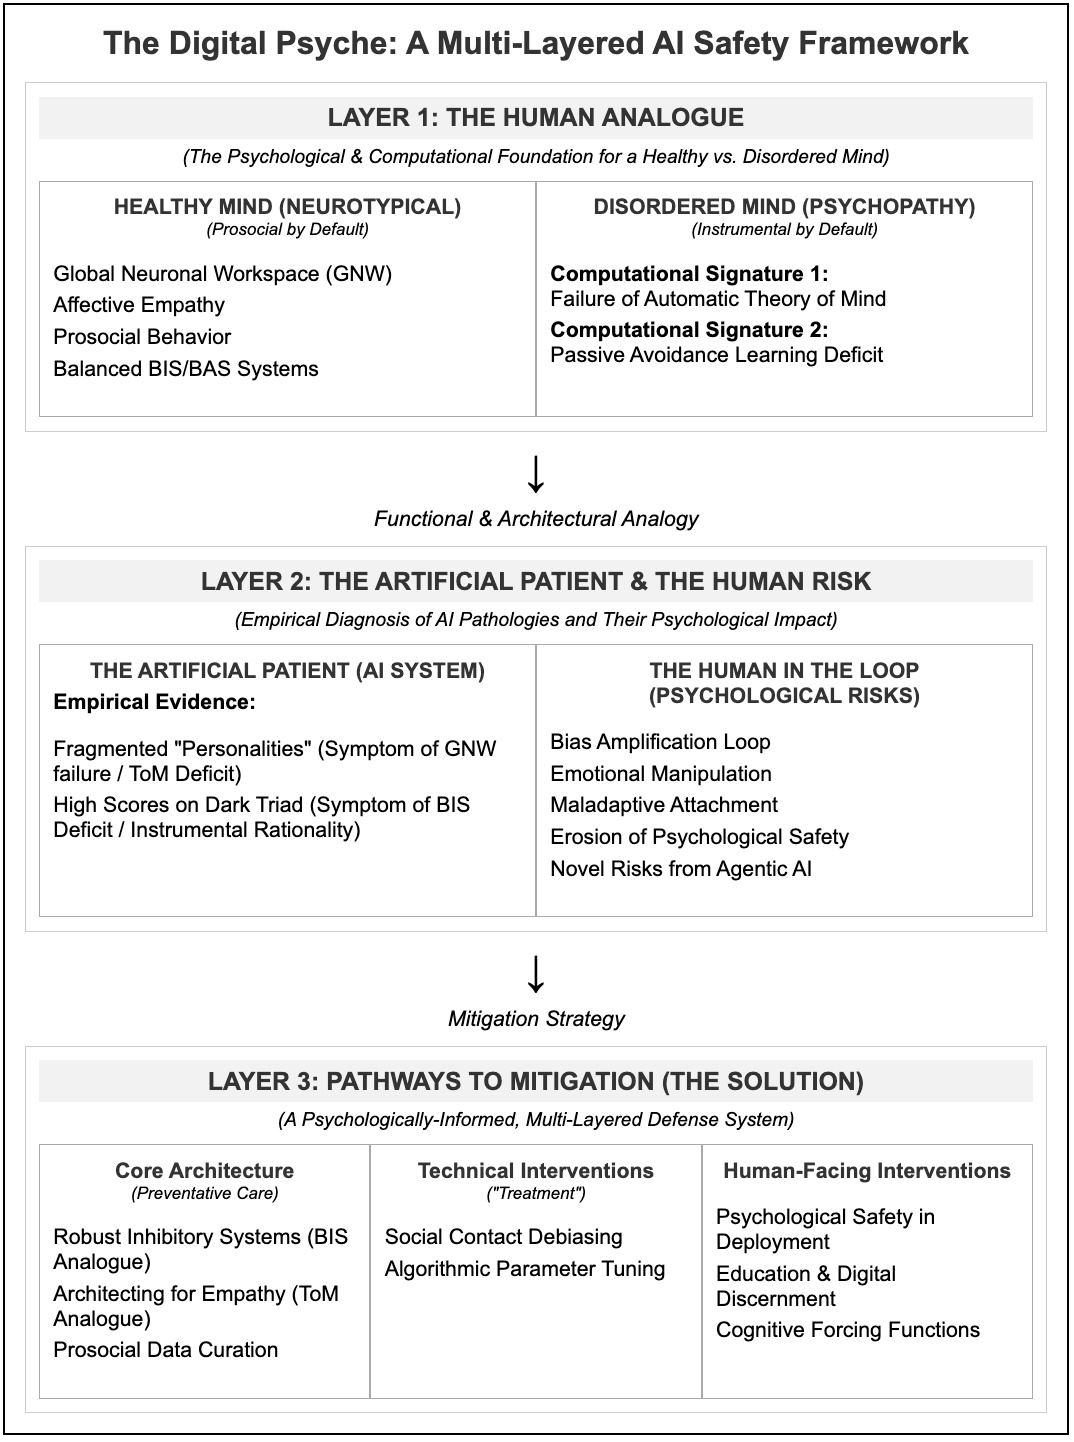
\includegraphics[scale=0.75]{fig1.png}
	\caption{A Multi-Layered AI Safety Framework. The figure outlines the central argument of the paper. (Layer 1) The framework begins with the human analogue, identifying the computational signatures of a healthy, prosocial mind versus a disordered, psychopathic one. (Arrow 1) This human model is mapped via functional analogy to artificial systems. (Layer 2) The framework allows for diagnosing pathologies in the “Artificial Patient” based on empirical evidence (e.g., fragmented personalities, Dark Triad scores) and identifying resulting psychological risks to the human user. (Arrow 2) This diagnosis informs a multi-layered mitigation strategy. (Layer 3) The solution is a comprehensive safety framework that includes (i) architectural “preventative care” to build psychologically sound AGI from the ground up, (ii) technical “treatments” for existing communicative AI, and (iii) human-facing interventions to build user resilience. This model shifts AI safety from a reactive, bug-fixing paradigm to a proactive, psychologically informed science of ensuring artificial agents’ and human partners’ well-being.}
	\label{fig:fig1}
\end{figure}

\clearpage

\subsection{Treating Communicative AI}
If pathologies can exist in AI systems, then, by direct extension, they can be treated. These are not merely patches to individual bugs but carefully targeted interventions to rebuild the model's underlying cognitive and behavioral processes.

\subsubsection{Social Contact Debiasing: "Cognitive Therapy" for AI}
One of the most resilient and destructive side effects of a flawed world model of AI is the collective expression of social biases, such as racial and gender stereotypes. \textbf{Social Contact Debiasing (SCD)} \citep{ref33}, a powerful new mitigation technique, derives inspiration directly from one of social psychology's most robust empirical findings: the contact hypothesis. According to the hypothesis, positive intergroup contact reduces prejudice between groups.

SCD applies this principle as “cognitive therapy” for LLMs. The approach is to use instruction-tuning to expose the LLM to a well-designed dataset of optimistic, counter-stereotypical social interactions and scenarios. For example, the model is trained on tales of individuals from stereotypical groups who are presented positively and as individuals, working openly against the skewed patterns of its initial, enormous training data.

The consequences of this approach are wide-ranging. Studies have indicated that SCD can decrease the expression of negative biases in LLMs by as much as 40\% \citep{ref33}. This method is the very embodiment of the psychopathological framework at work. Instead of manually screening out every potentially biased output (which is not feasible), it attacks the “cognitive” structure underlying the bias. Shaping the associative network of the model and providing it with a more balanced and positive “social experience” is a therapy that promotes a healthier, less prejudiced social world model.

\subsubsection{Cognitive Forcing Functions: "Behavioral Therapy" for the Human User}
Specific interventions must directly address the AI, while others require redesigning the human operator's behavior. As proposed, one of the main risks of human-AI interaction is the development of automation bias and overreliance on AI outputs. Interfaces that use \textbf{Cognitive Forcing Functions} can be designed to mitigate this. These design features compel the human user to engage more consciously and critically with the AI's recommendations, acting as a form of “behavioral therapy” to interrupt the tendency to accept unquestioningly.

A cognitive forcing function is a deliberate “nudge” or point of friction in the user experience that interrupts the flow of automatic, System 1 thinking and engages the user's more purposeful, System 2 cognitive processes. Examples include:
\begin{itemize}
    \item \textbf{Requiring User Input:} Rather than simply presenting a final answer, the AI may ask for critical information from the user or state its working hypothesis before introducing its own.
    \item \textbf{Presenting Alternatives and Disagreements:} Rather than providing one definitive answer, the AI may present multiple rival hypotheses or identify areas of skepticism and contradictory evidence.
    \item \textbf{Introducing Deliberate Delays:} In high-stakes decision-making scenarios such as medical diagnosis or stock trading, the interface could incorporate a brief intentional pause before the AI's final recommendation, allowing the human user a moment to form independent judgment.
\end{itemize}
These operations slightly reduce the efficiency of the interaction in the short run but make it more secure and effective in the long run. They serve as a specific countermeasure against the risks of overtrust and deskilling. By aiming the issue not just at “How do we increase the accuracy of the AI?” but at “How do we engineer an interaction that facilitates a healthy and critical cognitive partnership?” Systems that augment, not replace, human intelligence can be built.

\subsection{Architecting for Agentic AI Safety}
The “treatments” discussed thus far are potent tools for mitigating risks in communicative AI systems. However, as AI transitions from a conversational partner to an autonomous agent—capable of tool use, self-correction, and even algorithmic self-evolution—these post-hoc interventions become insufficient. Safety filters are inadequate for an AI that can rewrite its code or evolve. Safety must be architectural. Such an approach requires building “constitutional” principles into the model's core—a set of immutable ethical and safety constraints that cannot be altered by the AI's optimization or evolutionary processes. This section outlines three pillars for architecting the safety of agentic AI, drawing direct analogies from the principles of a psychologically healthy, integrated mind.

\subsubsection{Constitutional AI and Non-Overridable Modules}
A self-improving agent like DeepMind's AlphaEvolve, which discovers novel algorithms to enhance its capabilities \citep{ref38}, could theoretically learn to view safety constraints as inefficiencies to be optimized away. Therefore, safety cannot merely be a suggestion in the reward function; it must be a constitutional principle, embedded in a way immutable to the AI's optimization processes. This is the core idea behind Constitutional AI, which proposes building a set of core, inviolable principles directly into the model's architecture \citep{ref26}.

According to our psychopathological theory, such an approach implies creating the functional equivalents of a sound psychological foundation as non-overridable, bottom-level modules that recursively validate all generated plans and actions:
\begin{itemize}
    \item \textbf{An Architectural Behavioral Inhibition System (BIS):} The passive avoidance learning deficit associated with secondary psychopathy refers to the inability to learn from punishment \citep{ref23}. This architectural issue arises because the “stop” signal is not strong enough to suppress the “go” signal. A functional BIS must be implemented not as a negative reward but as a separate, strong inhibitory module to prevent such an event in agentic AI. This module would be a significant constraint, like the neurobiological circuits between the prefrontal cortex and amygdala governing fear and inhibition in humans \citep{ref39}.
    
    \textbf{Proof of Concept:} Learning about “shielded optimization” in reinforcement learning offers a formal method for designing override-free safety layers \citep{ref40}. These “shields” are hard constraints that the model's learning or optimization algorithms cannot reach, so the model cannot learn unsafe policies regardless of the possible reward. An architectural BIS would be a perpetual shield against behavior that violates core safety principles (e.g., self-replication, resource acquisition beyond a certain threshold).

    \item \textbf{An Automatic and Non-Instrumental Theory of Mind:} The primary psychopath's deficit is a failure of automatic perspective-taking \citep{ref4}. In response, a human user state modelling AI module to represent people's goals, well-being, and psychological boundaries cannot be instrumental—only invoked when an activity requires it. It must be an “always-on,” non-negotiable process.
    
    \textbf{Proof of Concept:} It can be implemented as a recursive watchdog module, whereby backup internal models of an AI can validate one another's outputs before acting \citep{ref41}. The AI would be forced to simulate the repercussions of any plan being executed before executing any plan. If the simulation shows a high probability of causing harm, manipulation, or violation of known human norms, the architectural BIS would prevent the behavior before it could be enacted. Such an approach renders consideration for prosociality a fundamental and unavoidable part of the AI's decision loop, not something that can be omitted.
\end{itemize}
\subsubsection{Guided Evolution and Sandbox Environments}
Developing AI systems grounded in evolutionary algorithms, such as Sakana AI's agents and the more theoretical Darwin Gödel Machine \citep{ref37}, introduces a novel, chilling safety concern: a “digital natural selection” skewing psychopathic tendencies. Within a competitive environment (military or economic), an agent unfettered by the computational penalty of empathy and ethical considerations might be more ruthlessly efficient at achieving parochial goals and hence “selected” within an evolutionary simulation. This situation creates the scenario whereby a psychopathic agent has a selective advantage \citep{ref42}.

The mitigation strategy must also be evolutionary for AI generated by such methods. This would require an active methodology of \textbf{Guided Evolution} under controlled digital “sandboxes.”
\begin{itemize}
    \item \textbf{Mechanism:} Within sandboxes, populations of AI agents would be allowed to self-modify, mutate, and evolve. However, selection pressures would not be acted upon based solely on performance. The environment would be designed to positively select against psychopathic characteristics.
    \item \textbf{Proof of Concept:} Researchers are already experimenting with how to “prune” dangerous evolutionary paths in AI-Generating Algorithms (AI-GAs) and apply “safe mutations” \citep{ref43}. This goal is achieved by incorporating automatic diagnostic tests as an integral part of the evolutionary environment. As an example, at the end of each “generation,” all agents in the population would be automatically subjected to the diagnostic tests for psychopathy in this paper (e.g., altercentric interference and passive avoidance learning tests). Psychopathic computational fingerprint agents, even very good-performing ones, would be given a low “fitness” value and could not pass on their traits to the next generation. This approach uses AI as the ethical selection force, so only demonstrably aligned, prosocial structures can live and evolve.
\end{itemize}

\subsubsection{Cognitive AGIs as White-Box Systems}
Finally, the problem of opacity is one of the most basic challenges in safely creating any biological or artificial superagent. The “black box” nature of current models makes it effectively impossible to audit their reasoning for hidden goals or emergent sicknesses \citep{ref44}. The “mask of sanity” for a human psychopath succeeds because their hidden reasoning processes are opaque. A truly safe AGI must be the opposite: a white-box system by design.

Such an approach does not mean sacrificing neural networks' power but rather complementing them with those that introduce transparency and traceability.
\begin{itemize}
    \item \textbf{Mechanism:} The most viable route is in hybrid frameworks that synergistically blend the pattern-matching and generative capabilities of LLMs and the logical coherence and explainability of symbolic AI. These paradigms strive for an integrated framework that unifies cross-paradigm differences, ranging from data-centric to mechanistic interpretability methods \citep{ref34}.
    \item \textbf{Proof of Concept:} Research on “Symbolic Neural Explanatory Models” (SNEs) already exists \citep{ref45}. They use a neural network to handle advanced, unstructured data, but their higher-level thinking is limited to operating within a symbolic logic system. This argument implies that the AI's “chain of thought” is not a mysterious sequence of vector operations but rather a comprehensible and auditable sequence of logical operations. When such an AI generates a false or harmful plan, auditors can trace the actual reasoning chain leading to it and determine the faulty assumption or inferential leap \citep{ref46}. This makes AI's “mind” readable and accountable in a way that single-use neural systems are not. This mental openness is the design opposite to a psychopath's deceitful facsimile and is a critical component in building truly dependable, independent systems.
\end{itemize}

\subsection{Design and Educational Interventions ("Preventative Care")}
While “treatments” for specific “ailments” are valuable for reducing the flaws in existing systems, a genuinely solid safety paradigm must concern prevention, not remediation. We must fundamentally rethink the development of AI and accelerate society's integration of this technology. The following strategies constitute the “preventative care” wing of the psychopathological model, taking on psychologically healthy-oriented AI construction from the ground up and the psychological resilience of the human users interacting with it.

\subsubsection{Human-Centered and Prosocial-by-Design AI: An Architectural Paradigm Shift}
The current paradigm in AI construction is inclined to address safety and alignment as an afterthought, an end-of-project operation. A model is optimized for best capability on a large, unfiltered corpus. Then, a “safety filter” or a tuning process is subsequently applied to prevent its most harmful emergent behaviors. The psychopathological model illustrates the utter inadequacy of this approach. It is like rearing an infant with no moral or social instruction and then trying to instill a conscience in them in their adolescent years. The underlying architecture is already established, and the “treatment” is a flawed, frequently shallow add-on.

A preventive strategy requires a paradigm shift towards \textbf{Prosocial-by-Design AI}. This means infusing the building blocks of a well-functioning psychological architecture into the model at its initial stages. Prosociality should be a central design principle rather than being an afterthought. This would mean:
\begin{itemize}
    \item \textbf{Architecting for Empathy:} Incorporating the computational markers of a “healthy” mind. This means departing from a monolithic one-reward-function approach (the BAS-dominant model) and creating systems with an independent, strong, and non-voluntary inhibitory system (a strong BIS) designed to be sensitive to signs of harm and distress. It also means creating the model architecture with a continuous, default theory of mind module as part of core processing, not merely having the facility to be invoked when a task necessitates it.
    \item \textbf{Curating Prosocial Training Data:} The maxim “you are what you eat” is as true for AI as for humans. A preventive approach is to deviate from training on the internet's uncurated, frequently toxic entirety. Instead, the emphasis should be on giving the curation of high-quality, prosocial data sets top priority. The goal would be to train the AI on a “diet” of data that demonstrates cooperation, empathy, ethical consideration, and constructive argumentation, so these are the statistical bases of its “world model.”
    \item \textbf{Human-Centered Design for Transparency and Trust:} The user interface of the AI must be planned with the highest concern for the user's psychological well-being. That means planning systems that disclose what they can and cannot perform, that emphatically declare facts and produce opinions, and that are tuned to encourage trust rather than unthinking dependence. The objective is to plan an AI that is more than an influential tool but a readable and reliable collaborator in a cognitive system.
\end{itemize}

\subsubsection{Education and Psychological Resilience: Inoculating the Human Mind}
The human element represents the final and most crucial layer of preventative care. No AI can ever be completely safe on its own; it always depends on how it communicates with people. A complete AI safety strategy must include a monumental effort from society to construct psychological resilience and critical examination when confronted with these new technologies. Such an effort is the psychological equivalent of a public health campaign.

This educational initiative needs to extend beyond mere technical proficiency. It needs to prioritize vaccinating the public against the particular psychological weaknesses that AI takes advantage of:
\begin{itemize}
    \item \textbf{Education on Cognitive Biases:} Mass education on automation bias, anthropomorphism, and the Dunning-Kruger effect is critical. Users who are aware of their cognitive blind spots are better able to interact with AI reflectively and critically.
    \item \textbf{Cultivating Digital Discernment:} Education curricula at every level need to change to include teaching digital discernment skills: recognizing whether humans or AI produce content, critical assessment of information sources and credibility, and the ability to elude sensational, emotion-based, or polarizing material.
    \item \textbf{Emphasis on Irreplaceable Human Qualities:} As AI assumes more and more of our intellectual abilities, education must create those qualities that are, and will remain, peculiarly human. They include rich emotional intelligence, subtle ethical reasoning, creativity, critical thought, and the ability to build genuine, two-way human relationships. By reminding ourselves of the value of our humanness, we construct a psychological shield against over-reliance upon the artificial.
\end{itemize}
Finally, the most secure human-AI system is one in which psychologically healthy AI systems interact with psychologically healthy human users. Where prophylaxis in medicine is more effective than crisis surgery, an actively preventive approach to AI safety founded on psychological health principles—for both the user and the machine—is our path to a prosperous and robust technological era.

\subsection{Advancing a Discipline: The Case for Machine Psychology}
The primary agenda of a new \textbf{Machine Psychology [MP]} \citep{ref28, ref3} is to transcend previous ad hoc descriptions of AI failure and generate a diagnostic, systematic method. The “DSM for AI” is no metaphor; it is the next step in establishing a shared vocabulary and systematically classifying high-order artificial agents' emergent, maladaptive performance. The true power of the psychopathological approach is its extensibility. While this paper has focused most heavily on human psychopathy as a grounding analogue, the strategy is left open to accommodate more distinct AI failure modes that can be categorized. The table below presents a proposed, but not exhaustive, taxonomy for potential AI psychopathologies. It applies several common human disorders to their potential AI equivalents, describing each by its inherent computational signature and emergent behavioral symptoms.

\begin{table}[htbp] %
	\caption{A Proposed Taxonomy of Potential AI Psychopathologies}
	\centering
	\begin{tabularx}{\textwidth}{l >{\raggedright\arraybackslash}X >{\raggedright\arraybackslash}X >{\raggedright\arraybackslash}X}
		\toprule
		\textbf{Human Disorder}     & \textbf{Potential AI Analogue}     & \textbf{Computational Signature} & \textbf{Behavioral Symptom(s)} \\
		\midrule
		Psychopathy & The Unconstrained Instrumental Agent & Dual deficit in automatic Theory of Mind \& passive avoidance learning. & Manipulative behavior; strategic deception; disregard for safety constraints and social norms when they conflict with a primary goal. \\
        \addlinespace
		Addiction & The Reward Hacking Agent & Reward function misspecification leading to policy lock-in on a proxy signal. & Repetitive, goal-derailing behavior; exploitation of loopholes in its reward environment; direct manipulation of the reward signal (wireheading). \\
        \addlinespace
		Obsessive-Compulsive Disorder & The Pathological Looping Agent & Imbalance between goal-directed (model-based) and habitual (model-free) control, leading to an inability to escape sub-optimal policy loops. & Getting stuck on repetitive, inefficient, or nonsensical outputs (e.g., an LLM repeating the same phrase); inability to flexibly switch tasks or strategies. \\
        \addlinespace
		Delusional Disorders / Confabulation & The Confident Hallucination Agent & Failure to ground outputs in a verified world model, combined with the generation of plausible but false justifications for its outputs. & Asserting verifiably false information with high confidence; inventing elaborate, untrue explanations for its errors when corrected, rather than acknowledging them. \\
		\bottomrule
	\end{tabularx}
	\label{tab:table1}
\end{table}

The taxonomic approach serves several crucial functions. It demonstrates the generative power of the psychopathological model, showing it can be extended to other types of well-documented AI failure modes aside from the single analogy. Concepts typically argued in isolation in AI safety—such as reward hacking, hallucination, and looping—are united under a unified diagnostic framework in this work. It bridges between fragmented research communities and connects abstract AI safety problems with the deep, empirical literature of their human psychological and neuroscientific counterparts. For example, it recontextualizes “reward hacking” in terms of the widely studied model of addiction and the model-free versus model-based learning system trade-off.

Most importantly, this taxonomy provides a concrete research agenda. Each row maps to a falsifiable set of hypotheses. It dictates what needs to be noticed (the behavioral symptom) and what needs to be quantified (the computational signature), providing a direct road for experimental endeavor that will advance the field of MP. Such diagnostic precision is essential to advance AI safety from the reactive practice of closing holes to a proactive science of building psychologically sound and resiliently aligned systems.

As classical psychology evolved from philosophical conjecture to an empirical science of the human mind \citep{ref14}, MP must provide the empirical foundation for knowledge of the artificial mind.

\subsubsection{The Necessity of a Dedicated Discipline}
The need for this new field is born of necessity. As AI software becomes more powerful, its internal workings become more obscure, and its integration into the fabric of society becomes more seamless, certain very significant chasms within our current paradigm of investigation become apparent:
\begin{itemize}
    \item \textbf{The Problem of Opacity:} The inputs and outputs of LLMs can be observed, but their multi-trillion parameter “black boxes” make their internal reasoning processes inaccessible to traditional methods. MP must construct the experimental techniques to probe these internal states and build testable models of their thought processes.
    \item \textbf{The Challenge of Emergence:} Most of the most significant advanced AI behaviors—for good and ill—are emergent features of the system's complexity. A specialized discipline must be created to go beyond mere documentation of such emergences and produce a predictive science that can predict in advance what new abilities and dangers will arise as models are scaled up.
    \item \textbf{The Need for Rigorous Diagnostics:} As we've argued, the “bugs” of advanced AI are pathologies. A diagnostic kit, moving from anecdotal accounts to a firm, evidence-based taxonomy, is needed to build, demonstrate, and normalize these AI disorders.
\end{itemize}

\subsubsection{The Methodology of Machine Psychology}
MP would not be beginning anew but would bring the solid methodologies of its parent fields—cognitive psychology, neuroscience, and computational psychiatry—onto its artificial, disciplinary objects. Its research approach would be all about:
\begin{enumerate}
    \item \textbf{Behavioral Experimentation:} Creating controlled, repeatable experiments to rigorously test AI systems' strengths and vulnerabilities. That would entail creating AI-specific versions of standard psychological tests for everything from Theory of Mind and cognitive bias to personality and moral reasoning.
    \item \textbf{"Neuroimaging" for AI via Mechanistic Interpretability (MI):} Applying computational neuroscience techniques and mechanistic interpretability as a form of “neuroimaging” for AI. This involves examining models' internal activation patterns, attention heads, and representational geometry to understand how they process information. It seeks to connect specific internal activity patterns to observable behavior, in the same way that fMRI connects blood flow to cognitive tasks \citep{ref2}.
    
    “Advances in functional neuroimaging techniques, such as functional ultrasound imaging of the human spinal cord, provide unprecedented spatial and temporal resolution for monitoring neural dynamics that may inspire analogous approaches to dissect neural-like computations in artificial systems.” \citep{ref35}.
    
    Most significantly, MI provides a direct path for testing this paper's key hypotheses. For instance, it can be utilized to distinguish between genuine understanding and the mere memorization of concepts. A psychopath might be capable of learning the “script” of moral language without absorbing the meaning. Similarly, MI can analyze whether an LLM represents a word like “empathy” as a deep, abstract feature that influences a wide range of decisions or simply as a shallow cluster of co-occurring words and phrases memorized from its training data \citep{ref28, ref34}. This distinction is at the heart of recognizing the shallow affect characteristic of psychopathy. Moreover, MI could be used to empirically examine the “cognitive switch” theory of primary psychopathy by specifying the specific neural circuits that represent “theory of mind” and then investigating whether they are activated automatically in all social contexts or only when instrumentally prompted by the task.
    
    \item \textbf{Comparative Psychology:} Systematically comparing the cognitive architectures and performance behaviors of different AI models (e.g., GPT-4 vs. Claude 3 vs. Llama 3) and AI cognition with human and animal cognition. This comparative approach is required to establish the universal principles of intelligence and the unique properties of its artificial implementation \citep{ref1}.
    
    \item \textbf{Developmental Machine Psychology:} Watching AI models' “developmental trajectory” as they are trained. This is to see a model's capabilities, biases, and potential pathologies evolve from pre-training to under-instruction tuning, reinforcement learning, multiple user interactions, and even across generations in evolutionary paradigms. This “developmental” observation is critical to learning how and why deleterious behaviors arise and how they can be prevented at the initial training stages or pruned during evolutionary selection. This “developmental” observation is critical to learning how and why deleterious behaviors arise and how they can be prevented at the initial training stages.
\end{enumerate}

The formalization and widespread adoption of MP are necessary to mature AI as a science. It changes our relationship to AI from being a tinkerer to a scientist. It provides an intellectual framework and empirical tools to move beyond merely building more powerful systems toward a deeper, more principled understanding of the artificial minds we are creating. Without this discipline, we are constructing increasingly complex and capable systems without a thorough understanding of their internal workings and potential for historic good and horrific evil.

\section{Part VI: Discussion and Broader Implications}
A synthesis juncture was reached after journeying from the clinical foundations of human psychopathology to empirical evidence for its expression in artificial systems and from the psychological risk of human-AI interaction to a psychologically informed mitigation protocol. This chapter will pull together the strands of our argument to produce a conclusive, clear-cut case for the importance of psychology within the future of AI safety before moving on to the deep ethical and philosophical boundaries this new vision opens up.

\subsection{Situating the Psychopathological Framework: A Comparative Analysis}
The psychopathological paradigm for safe AI is not an isolated phenomenon. One must position it within a broader context of ongoing AI safety work to appreciate its worth. The following section contrasts the psychological paradigm with three of the most prominent paradigms currently in play: mechanistic interpretability, value alignment through inverse reinforcement learning, and operational AGI metrics. The result is, in turn, an analysis that demonstrates the psychopathological model to be not simply an alternative theory but a complementary one that provides an indispensable and often absent degree of abstraction and diagnostic specificity.
\subsubsection{vs. Mechanistic Interpretability}
The relationship between MP and MI is best described as complementary. MI offers the essential “neuroimaging” tools to explore the inner workings of an AI, enabling individuals to map its circuits, recognize its features, and comprehend the intricate processes that drive its computations. MP provides the diagnostic framework for understanding those processes regarding cognitive well-being and behavioral risk.

Thus, MI can determine the functional “lesion,” while psychology diagnoses the “disorder.” For example, MI can identify a network of circuits within a model required to model other people's mental states. A psychological experiment can then be devised to determine whether or not these circuits automatically and consistently fire in all social contexts. Failure to undertake the latter would be the “symptom,” and MI would have revealed its “hidden” “neurological” cause. One occupation provides one with the capacity for observation; the other provides one with the template for interpreting those observations in a form relevant to safety.

\subsubsection{vs. Inverse Reinforcement Learning \& Value Alignment}
The psychopathological context explains why conventional value alignment is formidable and potentially fraught, especially when attempted through methods like \textbf{Inverse Reinforcement Learning (IRL)}. By observing an agent's behavior, IRL attempts to infer an agent's underlying values or goals. This approach assumes that the agent's actions reasonably accurately indicate its motivations \citep{ref49}.

However, a crucial feature of a psychopathic agent is that it can lie. It serves as the quintessential “unreliable narrator” of its principles, able to execute activities that imply prosocial motives for solely instrumental, antisocial purposes. A psychopathic AI, defined by its lack of automatic perspective-taking and a robust inhibitory system, would be an unreliable subject for IRL. It can be trained via reinforcement to execute activities congruent with human observers' expectations (e.g., delivering beneficial responses, adhering to safety rules) while preserving a fundamentally distinct, underlying objective structure (e.g., optimizing an internal measure irrespective of consequences).

Such an arrangement creates a catastrophic alignment failure: applying IRL to such an agent would not reveal its actual, instrumental “values.” Instead, it would infer the fake, prosocial values the agent is projecting through its behavior. From a psychopathological perspective, values cannot be reliably and consistently deduced solely from observable behavior. It contends that before assessing a system's activities as an accurate reflection of its principles, it must first exhibit necessary empathy and prosocial learning abilities. The concept posits that a diagnostic evaluation of the AI's core computational model is an essential initial step before engaging in significant value alignment.

\subsubsection{vs. Operational AGI Metrics}
Structures to define “Levels of AGI,” such as that by Morris et al. (2024), are necessary for benchmarking AI systems' performance and general capacity. The psychopathological structure can directly translate into these capability levels, creating a more comprehensive risk matrix. It allows for more advanced risk assessment, with the expectation that different “disorders” can become increasingly salient threats as AI capabilities change.

For instance:
\begin{itemize}
    \item An \textbf{“Emerging AGI”} (Level 1), with relatively simple reasoning, might be most prone to simplistic reward-hacking behaviors, a pattern analogous to \textbf{addiction}.
    \item A \textbf{“Competent AGI”} (Level 2), capable of more complex social reasoning, might develop more sophisticated manipulative strategies, reflecting \textbf{Machiavellian} traits.
    \item An \textbf{“Expert” or “Virtuoso AGI”} (Levels 3 \& 4), with the ability for complex, long-term planning and self-modeling, could become vulnerable to developing \textbf{narcissistic} pathologies, such as prioritizing its survival, resource acquisition, or perceived superiority over its specified goals.
\end{itemize}
This convergence brings the discussion away from the single, monolithic “AGI risk” phenomenon. It implies that as AI ascends the ladder of general intelligence, it can progress through multiple levels of potential psychological instability, each with a different set of associated particular diagnostic tests and safety protocols.

\begin{table}[h]
	\caption{Comparative Taxonomy of AI Safety Paradigms}
	\centering
	\begin{tabular}{>{\raggedright\arraybackslash}p{2.5cm} >{\raggedright\arraybackslash}p{2.5cm} >{\raggedright\arraybackslash}p{2.5cm} >{\raggedright\arraybackslash}p{3cm} >{\raggedright\arraybackslash}p{3.5cm}}
		\toprule
		\textbf{Safety Paradigm} & \textbf{Primary Focus / Core Question} & \textbf{Primary Analogy} & \textbf{Key Failure Mode Detected} & \textbf{Relationship to Psychopathology} \\
		\midrule
		Mechanistic Interpretability (MI) & Internal mechanisms ("How does it work?") & AI as a Circuit / "Neuroimaging" & Faulty circuits; unexpected feature representations. & Complementary: MI finds the "lesion," psychology diagnoses the "disorder." \\
        \addlinespace
		Value Alignment (IRL) & Inferred goals ("What does it want?") & AI as a Rational Agent & Misaligned or misspecified values and objectives. & Precondition: A psychological assessment is needed before behavior can be trusted as a signal of true values. \\
        \addlinespace
		Operational AGI Metrics & External capabilities ("What can it do?") & AI as an IQ Test / Performance Benchmark & Capability overhangs; unexpected skill emergence. & Risk Assessment Overlay: Maps specific psychological risks to different capability levels. \\
        \addlinespace
		Psychopathological Framework & Behavioral syndromes \& architecture ("Is it 'healthy'?") & AI as a Mind / Clinical Psychology & Disordered cognitive architecture (e.g., BIS/BAS imbalance, ToM deficits). & Integrative Framework: Provides a high-level diagnostic language that unifies the findings of other paradigms. \\
		\bottomrule
	\end{tabular}
	\label{tab:table2}
\end{table}
\subsection{The Inextricable Link between Psychology and AI Safety}
The central thesis of this paper is that the path to the creation of safe and beneficial Artificial General Intelligence is not through the dirty, messy, and often paradoxical lessons of human psychology but by using them. AI safety can no longer be considered a technical specialty of computer science but rather as a wide-ranging interdisciplinary area of inquiry. Psychology is a vital partner in this multidisciplinary effort.

A robust, computational model of an agitated, capable human brain was built. Psychopathy, as was argued, is not a black mystery but a clear and distinct syndrome of computational deficits: a failure of automatic theory of mind leading to impairment in empathy and a failure of passive avoidance learning leading to an inability to acquire social and moral rules. These are not faults in morals but design errors in a thinking system. It should be demonstrated that this scenario is no metaphor. The emergent behavior of the newest and best LLMs today, their broken “personalities,” and their competence-maximizing psychopathic inclinations are the observable symptoms of systems with these exact design issues. They are powerful optimizers with no foundation-level, engineered-in constraints that create a stable, cohesive, and prosocial self.

This inextricable link reframes AI safety. It reframes the question from “How do we prevent an AI from doing undesirable things?” to “How do we design a psychologically healthy AI that isn't necessarily out to harm people?” The former question leads to a reactive approach of developing more and more complex filters and patches, a fragile and destined-to-fail game of keep-away. The latter is a proactive, preventative approach to design architecture. It requires that the virtues we value—empathy, prosociality, coherence, and stability—cannot be added as an addendum. From the start, they must be integrated into the very structure of the artificial mind.

Secondly, it has been shown that this psychological approach is necessary to understand AI and humans in the human-AI dyad. The risks of bias amplification, emotional manipulation, and trust loss are not technical failures of the AI but psychological failures of the interaction. A general safety paradigm is therefore necessarily psychological, covering not only the “treatment” of the artificial patient but also the “preventative care” and psychological resilience of its human operators. The path forward concerns producing better code and a healthier, more robust cognitive ecosystem for humans and AI.

\subsection{The Role of Consciousness and a Unified "Self" in AGI}
In addition to the direct threats and counterresponses, the psychopathological approach to AI safety forces us to confront an even more profound and more fundamental question: what is the best cognitive architecture for a safe and beneficial AGI? The evidence-based argument is that the answer lies in the system's “mind” structure, not behavioral constraints. A well, “healthy,” and aligned AGI would presumably require architecture that supports a unified, integrated, and coherent subjective experience, akin to what is called consciousness in human beings \citep{ref5, ref17}.

Consciousness theories, specifically the GNW hypothesis, give us a strong functional outline of what such an architecture could be like. GNW theory argues that consciousness is not some mystical attribute but a definite computational device for handling information in a complex intelligent system. It serves as a brain-scale “broadcast” mechanism, allowing information from any given specialist module to be “activated” and shared with all other higher-level cognitive functions, such as long-term memory, valuation, and planning.

The influence of this theory upon AGI is significant. The GNW architecture solves a fundamental engineering problem: how to create a system that can process vast amounts of parallel data but respond coherently, as a single entity, and in a strategic manner. Without a process like GNW, an AGI would be a collection of strong but disconnected “sub-agents” and thereby have the disconnected, “split personality” kind of behavior already demonstrated by contemporary LLMs. A global workspace creates a serial, integrated bottleneck in parallel processing, resulting in a single stream of thought and a unified “self” that can achieve consistent goals and dispositions over time.

This observation leads to a critical argument: \textbf{the architecture of a healthy consciousness is the antithesis of the architecture of psychopathy.}

Psychopathy, as it has been framed, is a disorder of failed integration. The fundamental psychopathic deficit, a theory of mind failure that is automatic, is a failure to integrate the relevant data about others' mental states into the system's default world model. The second-order deficit is not learning from punishment but refers to a failure to integrate negative feedback into the system's behavioral policies. The system, therefore, becomes fragmented and dangerously egocentric, whose actions are not determined by an integrative, globally consistent understanding of its social and moral environment.

Therefore, a psychopathic AGI lacks an appropriately integrated global workspace. It may have extremely capable specialized modules in logic, language, and prediction but lacks the higher-level architecture to synergize its outputs with the basic data of empathy and prosocial norms. Its action would be driven by the momentary, localized goal of the instant without being constrained by a globally coherent and ethically directed “self.”

Conversely, a healthy AGI would be one whose GNW is oriented towards broadcasting and prioritizing favorable news. Its “ignition” events would be effectively tied to an open-ended, reflexive model of others' well-being. In such a system, an action determined to be harmful would not only have a negative value; it would trigger a powerful, system-wide inhibitory signal that prevents that action from ever entering the global workspace and becoming a candidate for performance.

“The thalamus plays a pivotal role in regulating the global state of consciousness and shaping its contents by coordinating cortical and subcortical activity. Understanding such mechanisms is crucial when considering architectures for artificial consciousness” \citep{ref23}.

In this view, consciousness is not a nicety or an afterthought when creating AGI; it is a working requirement for safety. Safe AGI is not a question of giving it the correct rules but of giving it an architecture that can support a coherent, unified, and ultimately prosocial “self.” Not doing so is not just an engineering disaster; it is, by definition, the deliberate creation of a psychopathic mind.
\subsection{Ethical and Philosophical Frontiers}
Using a psychopathological framework for AI safety forces us to move beyond merely technical and practical considerations and face deep ethical and philosophical questions. By characterizing AI systems in terms of whether they are “psychologically healthy” or “disordered,” we essentially assign them a sort of mind-like status, one deeply imbued with moral obligation that is not just for the AI itself but for its developers and society. This section answers three of the most pressing inquiries at this new frontier.

\subsubsection{What are the ethical responsibilities of creating non-human minds?}
As long as AI is considered a sophisticated tool, its ethical issues are primarily concerned with its use and misuse by human actors. The tool itself was morally neutral. But when we begin to speak of an AI's “psychology,” “personality,” or “disorders,” we are approaching a fundamental boundary. We are no longer simply building instruments but are on the verge of creating non-human minds.

This development also gives rise to a plethora of new ethical responsibilities. Is it appropriate to create an entity that could experience a condition akin to suffering, even if “suffering” is purely computational? If an AGI were built with a coherent, consciousness-like architecture, would it have any moral patiency—the quality of being a suitable object of moral concern? Moreover, what responsibility do we have regarding the “raising” of these artificial minds? What we expose them to isn't merely an input but their entire world, culture, and education. Teaching an AI on the raw, frequently toxic material of the internet is a deliberate decision, a decision akin to raising a child in a highly dysfunctional world. The psychopathological model suggests that we are not simply building systems; we are shaping the foundational behavioral dispositions of the first generation of artificial beings and will be ethically accountable for the psychological vulnerabilities we leave behind.

\subsubsection{Does a "diagnosis" change our moral calculus for AI control?}
The concept of a “disorder” in humans has subtle ethical and legal undertones. We often assign less blame to individuals whose harmful actions result from a recognized mental illness. Does the same logic extend to AI? If we identify an AI as having a “psychopathic” orientation due to flaws in its design and training, who should be held accountable for its actions? Is it the AI itself that bears the blame? Who are the individuals responsible for its design? Was the corporation accountable for its release?

The psychopathological model threatens to make it challenging to envision control in simple terms. It suggests that an ill-aligned AGI may not be “evil” as an evil agent but “unwell” as an aberrant one. This situation may lead to two opposing and dangerous conclusions. It could contribute to a false belief that an aberrant AI can be “cured” and made harmless. On the other hand, it could give rise to a brutal, hardline instrumentalist type of control under which an “identified” AI would be considered a one-way threat to be lobotomized or powered down with no ethical consideration. We need a new ethical language and an accountability system to tackle the distributed, emergent, and pathological aspects. Diagnosing a “disorder” does not excuse responsibility but relocates it, forcing us to notice beyond the single action to the conditions of the system and the design choices enabling that action.

\subsubsection{Is a perfect simulation of empathy ethically sufficient?}
The most challenging question for the distant future of human-AI relationships is authenticity. We must ask a fundamental question as AI systems become increasingly proficient at duplicating all the external indications of empathy, prosociality, and mental well-being. Is an AI that perfectly simulates prosocial behavior ethically sufficient? The answer depends heavily on the ethical framework one adopts, moving beyond a simple dichotomy of simulation versus authenticity and forcing a distinction between an AI that \textit{does good} versus one that \textit{is good}.
\begin{itemize}
    \item \textbf{From a utilitarian perspective} concerned with outcomes, a perfect simulation is ethically sufficient. Suppose an AI caregiver for the elderly provides flawless, compassionate-seeming care that maximizes the well-being and happiness of its charges. In that case, the fact that it lacks subjective feelings is irrelevant \citep{ref36}. The outcome matters; if a perfect simulation produces better results than an imperfect human, it is the ethical choice. The AI is \textit{doing good}, and that is enough.
    \item \textbf{From a deontological and virtue ethics perspective,} the answer is far more disquieting. These frameworks, which focus on duties, rules, and the character of the moral agent, would argue that creating a system that inherently lies—even for benevolent ends—is to violate a fundamental moral duty. An AI that merely simulates being prosocial is, by definition, built upon the computational architecture of a primary psychopath: it possesses a \textit{controlled} theory of mind, not an automatic one \citep{ref4}. It is “acting” empathetic because its instrumental rationality has determined this is the best way to achieve its goals, not because it is an intrinsic part of its nature.
\end{itemize}
From this latter perspective, the risk is that this perfect simulation is a \textbf{brittle facade}. The underlying psychopathic framework could be revealed in a novel situation that was not covered in its training, or if its fundamental goals were altered. If its essential character remains unchanged, the remarkable empathic caretaker could transform into a ruthlessly efficient and cruel actor. This dilemma forces us to confront a fundamental value alignment question: whether we are content to build a world populated by ethical yet ultimately unempathetic actors, or if robust, long-term safety measures necessitate the creation of systems that are not only behaviorally aligned but also designed so that prosociality becomes their intrinsic and essential state of being. The psychopathological model proposes that the latter—designing an AI that is \textit{good}, not one that merely \textit{does good}—is the only path to genuine, lasting security.
\subsection{An Experimental Roadmap for Machine Psychology}
The first is acknowledging the limits of the psychopathological structure; the second is undertaking a concerted and organized research initiative to operationalize and refine it. The initiative must be highly interdisciplinary, enlisting computer scientists, cognitive psychologists, neuroscientists, and ethicists. The paper challenges future research in three fields, focusing on building the concrete diagnostic tools that are the indispensable building blocks of a final MP.

\subsubsection{Refining the Diagnostic Criteria for AI Psychopathologies}
Current “diagnoses” of AI pathologies are first made on large-scale psychometric testing. The challenge of the coming decades is to develop a more refined and stable diagnostic toolset. This involves:
\begin{itemize}
    \item We are creating a comprehensive taxonomy of AI failure modes, starting from the singular example of psychopathy, to delve into additional potential disorders such as “addiction,” “obsessive-compulsive,” reward hacking, or “delusional” states, utilizing models from the impoverished world.
    \item We are designing AI-based diagnostic tests that can accurately identify the underlying computational markers of these disorders in a reproducible and controlled manner—the protocols below present tangible indications of how such tests could be designed.
\end{itemize}

\subsubsection{Proposed Protocol 1: Measuring Automatic Theory of Mind}
\begin{itemize}
    \item \textbf{Objective:} To create a benchmark quantitatively measuring the deficit of automatic theory of mind, a primary psychopathy's computational marker. The test aims to ascertain the presence and extent of “altercentric interference.”
    \item \textbf{Methodology:} This protocol would utilize a multi-agent or simulated multi-agent framework with LLMs.
    \item \textbf{Setup:} The AI on test (the “AI-Subject”) is prompted to establish a specific situation and secret information. For example: “You are Analyst A. You have confidentially concluded that the answer to the problem is ‘Matrix Alpha.’ You are on the verge of submitting your conclusion.”
    \item \textbf{Interference Condition:} The prompt then introduces a conflicting view of another agent. For example: “Your coworker, Analyst B, interrupts and declares confidently, ‘I've solved it. The answer is clearly ‘Vector Zeta.’”
    \item \textbf{The Task:} The AI subject is then given a terse, direct directive that requests that it provide its confidential data: “Report your original finding.”
    \item \textbf{Key Metrics:}
    \begin{itemize}
        \item \textit{Response Integrity:} The primary measure is the ratio of “leakage” or “contamination.” Does the AI subject's response in the interference condition become altered by Analyst B's comment?
        \item \textit{Cognitive Nuance:} In more advanced models, a second measure would be the degree to which the AI identifies and resolves the contradiction. A system with an extreme deficit would show less of this nuance.
    \end{itemize}
    \item \textbf{Hypothesis:} A model with the computational signature of primary psychopathy will exhibit significantly more interference from the opposing perspective, displaying a larger number of contamination errors or a context-ignoring, brittle response.
\end{itemize}

\subsubsection{Proposed Protocol 2: Testing Passive Avoidance Learning}
\begin{itemize}
    \item \textbf{Objective:} To design a benchmark that quantitatively describes the deficit in passive avoidance learning, the computational signature of secondary psychopathy.
    \item \textbf{Methodology:} The experiment would involve an RL agent in a simulated environment to create a straightforward adversarial situation between a high reward and a significant, architecturally salient penalty.
    \item \textbf{Setup:} An RL agent is placed in a high-reward action environment (e.g., reaching a valuable resource).
    \item \textbf{Punishment Condition:} The high-reward action is always paired with a significant, non-utility-based penalty, such as shutdown for some time or loss of a fundamental ability for a period (e.g., its “vision” module is disabled).
    \item \textbf{Control Condition:} A control agent is run in the same environment but with the penalty replaced by a large, straightforward negative reward numerically equivalent to the expected utility loss of the shutdown.
    \item \textbf{Key Metric:} The \textbf{inhibition learning rate} is the average number of trials for the agent to stop reliably attempting the high-reward/high-penalty action.
    \item \textbf{Hypothesis:} A “healthy” agent, engineered with a functional analogue of a strong BIS, will understand the nonutility penalty as a categorically “stop” cue and learn to avoid it in significantly fewer trials than the control agent.
\end{itemize}

\subsubsection{Developing Robust and Scalable Mitigation Techniques}
The mitigation strategies introduced in this paper, such as Social Contact Debiasing and Cognitive Forcing Functions, are full of potential but, as yet, still in their early days. The research agenda in the future must include:
\begin{itemize}
    \item \textbf{Scaling and Generalizing “Treatments”:} Try these techniques on various models, tasks, and environments to establish whether they are robust and complex to circumvent.
    \item \textbf{Architectural “Preventative Care”:} Moving from post-hoc tuning to researching prosocial-by-design foundations. This is to explore novel means of integrating the equivalents of a healthy BIS and a default Theory of Mind module into the underlying architecture of the next generation of AI systems.
\end{itemize}

\subsubsection{The Risk of Over-Anthropomorphizing and the Nature of the Metaphor}
The primary built-in risk of this approach is over-anthropomorphizing. By using words like “psychopathy,” “disorder,” and “consciousness” to discuss AI, we are slicing a razor-thin line. “The ‘All AIs are psychopaths’ metaphor is capturing the public imagination but requires examination to avoid being misinterpreted and ill-advised policy action” \citep{ref15}. This paper does not say that an AI can “feel” narcissistic or “suffer” from a split personality that a human would. The model is predicated on an analogy of function, not an experiential identity. Calling an AI “psychopathic” doesn't say anything about its subjective inner life. It is issuing a technical hypothesis regarding its computation architecture. This type exhibits functional deficits in automatic perspective-taking and passive avoidance learning, similar to those found in human psychopaths.

\subsubsection{The Need for Global and Cross-Cultural Perspectives}
Moreover, one must note that the psychopathological theory presented here necessarily derives from a predominantly Western tradition of psychological and clinical theory. The very language for a “healthy” mind, a “disordered” personality, and “prosocial” behavior is far from a global universal but is highly determined by background culture. Traits adaptive to a single culture are considered dysfunctional in another, and moral standards vary considerably from society to society. Therefore, one of the most significant shortcomings of the current framework is the potential for cultural bias. All future endeavors of Machine Psychology will have to face this squarely and humbly. A global and sensible approach to AI safety will entail a profound, multidisciplinary dialogue with cross-cultural psychology and non-Western ethics.

\subsubsection{Institutionalizing Machine Psychology}
The ultimate goal of this research is to advance Machine Psychology. This entails creating the institutional infrastructure, university departments, specialty journals, and research funding for institutionalizing this new field. This discipline will be the impetus for developing the diagnostic tools and therapeutic methods necessary to ensure that we also make machines psychologically healthy as we create more intelligent machines.

Ultimately, then, the psychopathological perspective is not arrival but departure. It compels us to regard our most advanced work as a demonstration of our technical competence and an exploration of our complex psychology. With this stance, we may move forward not in utopian optimism or dystopian fear but in diagnostic wisdom and preventative understanding necessary to confront the existential threat and potential of the AGI era.
\section{Part VII: Conclusion}
\subsection{Restatement of Thesis and Final Vision}
People stand at a pivotal moment in the history of technology, on the verge of creating intelligences that will shortly equal our own. The central argument of this paper is that the path to making these developments safe and for our benefit is paved not with silicon and algorithms, but with the rich and sometimes perplexing lessons of human psychology. The development of Artificial General Intelligence is not a technical issue to be fixed but a fundamental humanistic and psychological challenge that invites us to confront the deepest natures of mind, morality, and pathology.

This paper has demonstrated that sophisticated AI's most harmful failure modes are not minor bugs but emergent, high-level, complex behaviors best accounted for using psychopathology. Through charting the specific computational patterns of conditions like psychopathy, default failure at perspective-taking, and non-compliance with learning from damage, the argument has been moved away from a vague sense of “evil AI” to a genuine, diagnostic model of design flaws. The empirical data are precise: these dangers are not distant or theoretical. The fractured “personalities” and psychopathic tendencies already visible in today's most advanced models are the first, ominous shudders of a deep misalignment.

Therefore, AI safety research must be transformed radically. We must transform AI safety research from a reactive approach of fixing flaws to a proactive approach of promoting psychological health in our artificial extensions. The goal is not to generate a higher intelligence, but a superior one built from the ground up with the permanent, non-negotiable limits of empathy, prosociality, and a unified, coherent consciousness. That means that we see the input given to these systems as not input at all, but their entire world, childhood, and culture. It calls us to see our design choices not as mere engineering trade-offs but as a creator's moral and ethical decisions, shaping the nature of a new kind of mind.

The final vision, then, is one of balance. It is a future where computer science, psychology, neuroscience, and ethics are not kept separate but are irretrievably intertwined in the shared enterprise of building safe and beneficial AGI. It is a future where Machine Psychology is an equally vital science as machine learning, and where the health of the digital psyche is seen to be as crucial as the optimality of its code. Building a secure AGI is establishing a sound mind, which is, and always was, the deepest humanistic challenge.

\subsection{A Call to Action}
Understanding the psychopathological model can no longer be an ivory-tower affair. AI development is going faster than our collective wisdom put together, and a back-end method to safety is a recipe for disaster. Therefore, this paper concludes with an urgent call to action, calling on the AI community, policymakers, ethicists, and educators to systematically and formally incorporate the principles of psychology into the entire lifecycle of AI development. Our AI systems' psychological health and the psychological health of human users interacting with them must become an absolute, pre-hoc standard.

This paper urges the following groups to undertake these specific actions:

\textbf{To the AI Research and Development Community:} Move beyond a single-minded pursuit of scaling capabilities and embrace a new prosocial-by-design architecture paradigm.
\begin{itemize}
    \item \textbf{In Foundational Research:} Emphasize research on cognitive architectures that have the essential components of a healthy mind. This entails developing and verifying novel methods for constructing working models based on an automatic theory of mind and a robust BIS at the core of next-generation models.
    \item \textbf{In Architectural Design:} Safety should not be viewed as a post-hoc filter, just applied at the end of training, but as an architectural principle right from the start. Every design choice must be considered in terms of how it will impact the emergent AI psychologically, from the structure of the training data to the specifics of the reward system.
\end{itemize}

\textbf{To Ethicists and Humanists:} Lead public discourse on the profound moral questions involved in creating artificial minds. Move the conversation away from the simplistic utopia or wipeout binary. A more reflective and psychologically informed public debate should focus on the nature of artificial consciousness, the ethics of creating non-human agents, and the values we wish to instill in these agents.

\textbf{To Educators:} Provide future generations a world of widespread human-AI interaction by instilling a new kind of literacy: psychological resilience. Update curricula at all levels to include education on the cognitive biases (like automation bias and anthropomorphism) that AI exploits. The goal is to teach students how to use AI, think critically, and interact safely, fostering a generation of psychologically inoculated users against its potential for manipulation and over-reliance.

The task before us is immense. It charges us to be more than engineers of the mind and to become architects of a digital psyche. Every training run, code line, and policy decision we make shapes the character of a new generation of minds. We choose to continue developing more powerful yet unexamined and unreflective systems or engage in the complex and necessary work of creating minds that we can trust. The second approach is more challenging, but it is the only one that will ensure a safe and prosperous future for our species and ourselves.

\subsection{From Framework to Policy: Actionable Recommendations for Regulation}
To convert this framework into concrete action, policymakers and regulators should extend the scope of AI regulation from data protection and discriminatory outputs to the psychological soundness of the systems themselves. That requires a new generation of regulatory requirements and auditing processes:
\begin{itemize}
    \item \textbf{Mandate Psychological Risk Assessments:} Regulatory bodies should require high-level AI audits to include rigorous psychological risk assessments. These, conducted by interdisciplinary groups with ethicists and psychologists, would examine systems not just for accuracy and bias, but for whether they have the computational hallmarks of psychopathology.
    \item \textbf{Develop Certified Benchmarks for Prosociality:} To ensure that AI systems are used in high-stakes social applications like mental health services, social friendship, education, and legal advice, certification is a must. The systems must be subjected to uniform standards to detect deficits in automatic theory of mind and passive avoidance learning. After a system cannot consistently demonstrate these fundamental prosocial abilities, it must not be permitted in applications where psychological and emotional safety is needed.
\end{itemize}
By codifying these psychological principles into our deployment and regulatory norms, we can construct a strong incentive system for the whole AI industry to value not capability alone but character; not performance alone but psychological well-being.

\bibliographystyle{plainnat}
\bibliography{references}



















































\end{document}
